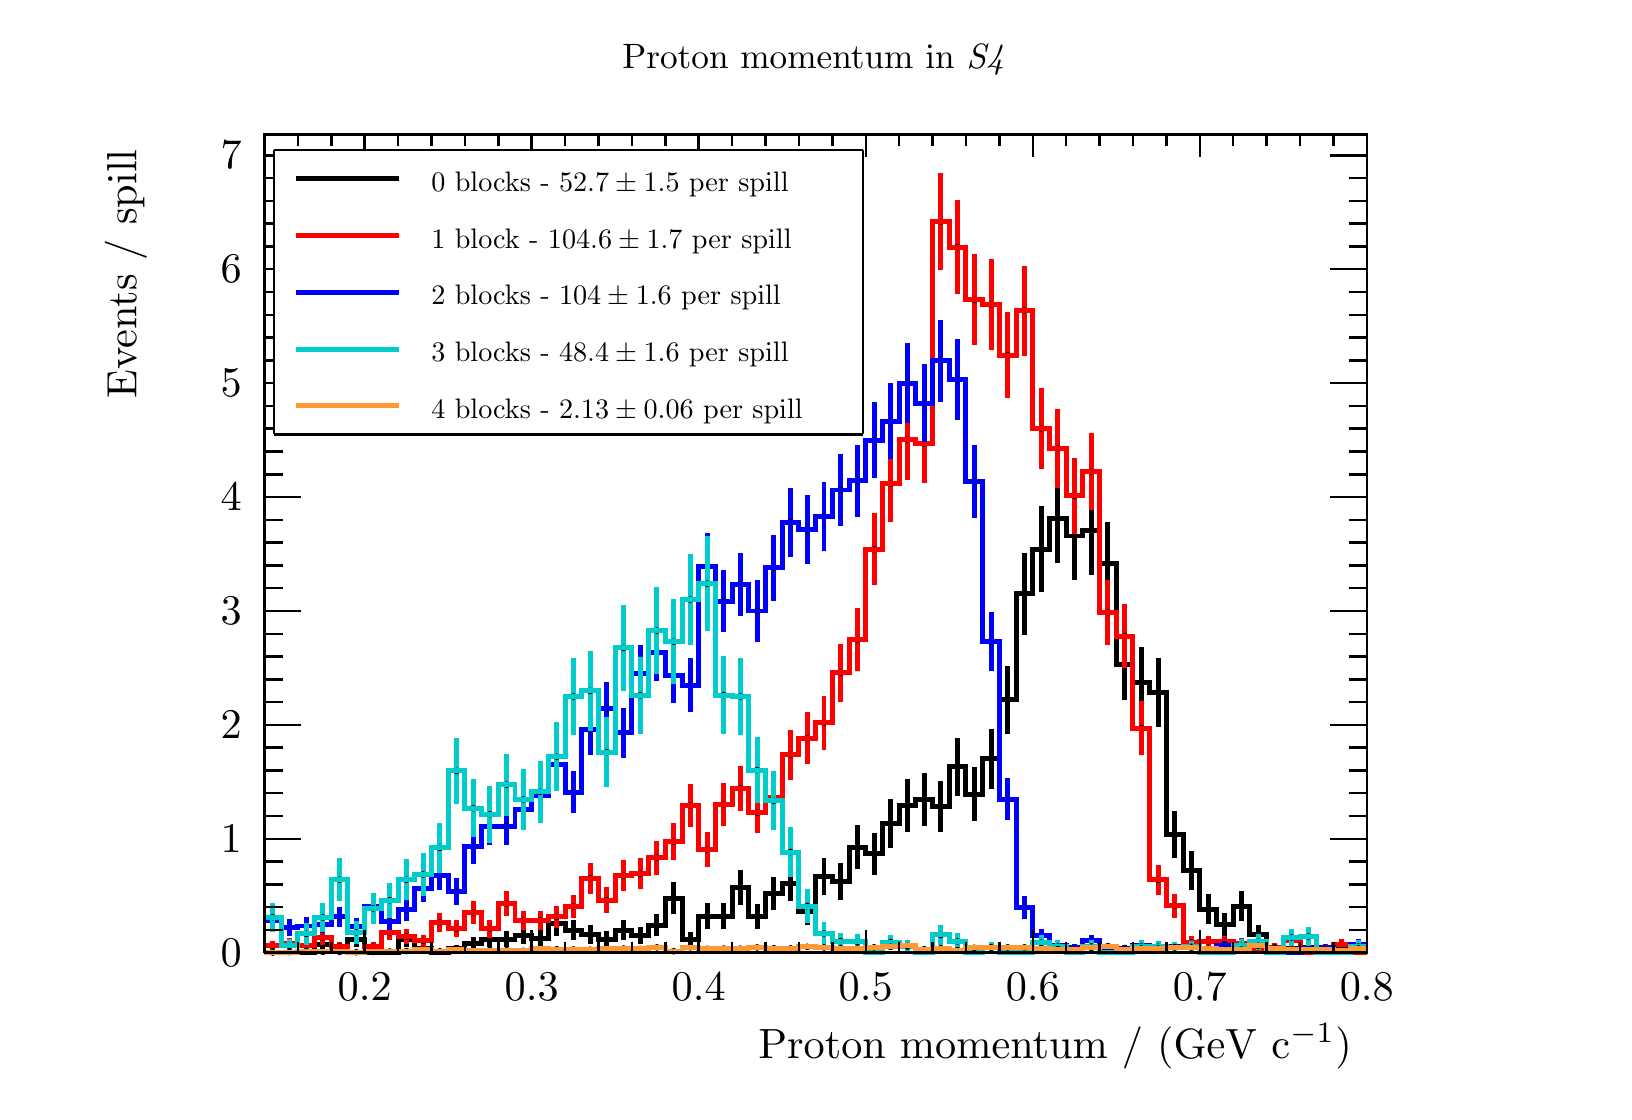
\begin{tikzpicture}
\pgfdeclareplotmark{cross} {
\pgfpathmoveto{\pgfpoint{-0.3\pgfplotmarksize}{\pgfplotmarksize}}
\pgfpathlineto{\pgfpoint{+0.3\pgfplotmarksize}{\pgfplotmarksize}}
\pgfpathlineto{\pgfpoint{+0.3\pgfplotmarksize}{0.3\pgfplotmarksize}}
\pgfpathlineto{\pgfpoint{+1\pgfplotmarksize}{0.3\pgfplotmarksize}}
\pgfpathlineto{\pgfpoint{+1\pgfplotmarksize}{-0.3\pgfplotmarksize}}
\pgfpathlineto{\pgfpoint{+0.3\pgfplotmarksize}{-0.3\pgfplotmarksize}}
\pgfpathlineto{\pgfpoint{+0.3\pgfplotmarksize}{-1.\pgfplotmarksize}}
\pgfpathlineto{\pgfpoint{-0.3\pgfplotmarksize}{-1.\pgfplotmarksize}}
\pgfpathlineto{\pgfpoint{-0.3\pgfplotmarksize}{-0.3\pgfplotmarksize}}
\pgfpathlineto{\pgfpoint{-1.\pgfplotmarksize}{-0.3\pgfplotmarksize}}
\pgfpathlineto{\pgfpoint{-1.\pgfplotmarksize}{0.3\pgfplotmarksize}}
\pgfpathlineto{\pgfpoint{-0.3\pgfplotmarksize}{0.3\pgfplotmarksize}}
\pgfpathclose
\pgfusepathqstroke
}
\pgfdeclareplotmark{cross*} {
\pgfpathmoveto{\pgfpoint{-0.3\pgfplotmarksize}{\pgfplotmarksize}}
\pgfpathlineto{\pgfpoint{+0.3\pgfplotmarksize}{\pgfplotmarksize}}
\pgfpathlineto{\pgfpoint{+0.3\pgfplotmarksize}{0.3\pgfplotmarksize}}
\pgfpathlineto{\pgfpoint{+1\pgfplotmarksize}{0.3\pgfplotmarksize}}
\pgfpathlineto{\pgfpoint{+1\pgfplotmarksize}{-0.3\pgfplotmarksize}}
\pgfpathlineto{\pgfpoint{+0.3\pgfplotmarksize}{-0.3\pgfplotmarksize}}
\pgfpathlineto{\pgfpoint{+0.3\pgfplotmarksize}{-1.\pgfplotmarksize}}
\pgfpathlineto{\pgfpoint{-0.3\pgfplotmarksize}{-1.\pgfplotmarksize}}
\pgfpathlineto{\pgfpoint{-0.3\pgfplotmarksize}{-0.3\pgfplotmarksize}}
\pgfpathlineto{\pgfpoint{-1.\pgfplotmarksize}{-0.3\pgfplotmarksize}}
\pgfpathlineto{\pgfpoint{-1.\pgfplotmarksize}{0.3\pgfplotmarksize}}
\pgfpathlineto{\pgfpoint{-0.3\pgfplotmarksize}{0.3\pgfplotmarksize}}
\pgfpathclose
\pgfusepathqfillstroke
}
\pgfdeclareplotmark{newstar} {
\pgfpathmoveto{\pgfqpoint{0pt}{\pgfplotmarksize}}
\pgfpathlineto{\pgfqpointpolar{44}{0.5\pgfplotmarksize}}
\pgfpathlineto{\pgfqpointpolar{18}{\pgfplotmarksize}}
\pgfpathlineto{\pgfqpointpolar{-20}{0.5\pgfplotmarksize}}
\pgfpathlineto{\pgfqpointpolar{-54}{\pgfplotmarksize}}
\pgfpathlineto{\pgfqpointpolar{-90}{0.5\pgfplotmarksize}}
\pgfpathlineto{\pgfqpointpolar{234}{\pgfplotmarksize}}
\pgfpathlineto{\pgfqpointpolar{198}{0.5\pgfplotmarksize}}
\pgfpathlineto{\pgfqpointpolar{162}{\pgfplotmarksize}}
\pgfpathlineto{\pgfqpointpolar{134}{0.5\pgfplotmarksize}}
\pgfpathclose
\pgfusepathqstroke
}
\pgfdeclareplotmark{newstar*} {
\pgfpathmoveto{\pgfqpoint{0pt}{\pgfplotmarksize}}
\pgfpathlineto{\pgfqpointpolar{44}{0.5\pgfplotmarksize}}
\pgfpathlineto{\pgfqpointpolar{18}{\pgfplotmarksize}}
\pgfpathlineto{\pgfqpointpolar{-20}{0.5\pgfplotmarksize}}
\pgfpathlineto{\pgfqpointpolar{-54}{\pgfplotmarksize}}
\pgfpathlineto{\pgfqpointpolar{-90}{0.5\pgfplotmarksize}}
\pgfpathlineto{\pgfqpointpolar{234}{\pgfplotmarksize}}
\pgfpathlineto{\pgfqpointpolar{198}{0.5\pgfplotmarksize}}
\pgfpathlineto{\pgfqpointpolar{162}{\pgfplotmarksize}}
\pgfpathlineto{\pgfqpointpolar{134}{0.5\pgfplotmarksize}}
\pgfpathclose
\pgfusepathqfillstroke
}
\definecolor{c}{rgb}{1,1,1};
\draw [color=c, fill=c] (0,0) rectangle (20,13.4957);
\draw [color=c, fill=c] (3,1.75444) rectangle (17,12.1461);
\definecolor{c}{rgb}{0,0,0};
\draw [c,line width=0.9] (3,1.75444) -- (3,12.1461) -- (17,12.1461) -- (17,1.75444) -- (3,1.75444);
\definecolor{c}{rgb}{1,1,1};
\draw [color=c, fill=c] (3,1.75444) rectangle (17,12.1461);
\definecolor{c}{rgb}{0,0,0};
\draw [c,line width=0.9] (3,1.75444) -- (3,12.1461) -- (17,12.1461) -- (17,1.75444) -- (3,1.75444);
\draw [c,line width=0.9] (3,1.75444) -- (3.21212,1.75444) -- (3.21212,1.75444) -- (3.42424,1.75444) -- (3.42424,1.75444) -- (3.63636,1.75444) -- (3.63636,1.75444) -- (3.84848,1.75444) -- (3.84848,1.75444) -- (4.06061,1.75444) -- (4.06061,1.75444) --
 (4.27273,1.75444) -- (4.27273,1.75444) -- (4.48485,1.75444) -- (4.48485,1.75444) -- (4.69697,1.75444) -- (4.69697,1.75444) -- (4.90909,1.75444) -- (4.90909,1.75444) -- (5.12121,1.75444) -- (5.12121,1.75444) -- (5.33333,1.75444) -- (5.33333,1.75444)
 -- (5.54545,1.75444) -- (5.54545,1.75444) -- (5.75758,1.75444) -- (5.75758,1.75444) -- (5.9697,1.75444) -- (5.9697,1.75444) -- (6.18182,1.75444) -- (6.18182,1.75444) -- (6.39394,1.75444) -- (6.39394,1.75444) -- (6.60606,1.75444) -- (6.60606,1.75444)
 -- (6.81818,1.75444) -- (6.81818,1.75444) -- (7.0303,1.75444) -- (7.0303,1.75444) -- (7.24242,1.75444) -- (7.24242,1.75444) -- (7.45455,1.75444) -- (7.45455,1.75444) -- (7.66667,1.75444) -- (7.66667,1.75444) -- (7.87879,1.75444) -- (7.87879,1.75444)
 -- (8.09091,1.75444) -- (8.09091,1.75444) -- (8.30303,1.75444) -- (8.30303,1.75444) -- (8.51515,1.75444) -- (8.51515,1.75444) -- (8.72727,1.75444) -- (8.72727,1.75444) -- (8.93939,1.75444) -- (8.93939,1.75444) -- (9.15152,1.75444) --
 (9.15152,1.75444) -- (9.36364,1.75444) -- (9.36364,1.75444) -- (9.57576,1.75444) -- (9.57576,1.75444) -- (9.78788,1.75444) -- (9.78788,1.75444) -- (10,1.75444) -- (10,1.75444) -- (10.2121,1.75444) -- (10.2121,1.75444) -- (10.4242,1.75444) --
 (10.4242,1.75444) -- (10.6364,1.75444) -- (10.6364,1.75444) -- (10.8485,1.75444) -- (10.8485,1.75444) -- (11.0606,1.75444) -- (11.0606,1.75444) -- (11.2727,1.75444) -- (11.2727,1.75444) -- (11.4848,1.75444) -- (11.4848,1.75444) -- (11.697,1.75444)
 -- (11.697,1.75444) -- (11.9091,1.75444) -- (11.9091,1.75444) -- (12.1212,1.75444) -- (12.1212,1.75444) -- (12.3333,1.75444) -- (12.3333,1.75444) -- (12.5455,1.75444) -- (12.5455,1.75444) -- (12.7576,1.75444) -- (12.7576,1.75444) --
 (12.9697,1.75444) -- (12.9697,1.75444) -- (13.1818,1.75444) -- (13.1818,1.75444) -- (13.3939,1.75444) -- (13.3939,1.75444) -- (13.6061,1.75444) -- (13.6061,1.75444) -- (13.8182,1.75444) -- (13.8182,1.75444) -- (14.0303,1.75444) -- (14.0303,1.75444)
 -- (14.2424,1.75444) -- (14.2424,1.75444) -- (14.4545,1.75444) -- (14.4545,1.75444) -- (14.6667,1.75444) -- (14.6667,1.75444) -- (14.8788,1.75444) -- (14.8788,1.75444) -- (15.0909,1.75444) -- (15.0909,1.75444) -- (15.303,1.75444) -- (15.303,1.75444)
 -- (15.5152,1.75444) -- (15.5152,1.75444) -- (15.7273,1.75444) -- (15.7273,1.75444) -- (15.9394,1.75444) -- (15.9394,1.75444) -- (16.1515,1.75444) -- (16.1515,1.75444) -- (16.3636,1.75444) -- (16.3636,1.75444) -- (16.5758,1.75444) --
 (16.5758,1.75444) -- (16.7879,1.75444) -- (16.7879,1.75444) -- (17,1.75444);
\draw [c,line width=0.9] (3,1.75444) -- (17,1.75444);
\draw [c,line width=0.9] (4.27273,2.03785) -- (4.27273,1.75444);
\draw [c,line width=0.9] (4.69697,1.89615) -- (4.69697,1.75444);
\draw [c,line width=0.9] (5.12121,1.89615) -- (5.12121,1.75444);
\draw [c,line width=0.9] (5.54545,1.89615) -- (5.54545,1.75444);
\draw [c,line width=0.9] (5.9697,1.89615) -- (5.9697,1.75444);
\draw [c,line width=0.9] (6.39394,2.03785) -- (6.39394,1.75444);
\draw [c,line width=0.9] (6.81818,1.89615) -- (6.81818,1.75444);
\draw [c,line width=0.9] (7.24242,1.89615) -- (7.24242,1.75444);
\draw [c,line width=0.9] (7.66667,1.89615) -- (7.66667,1.75444);
\draw [c,line width=0.9] (8.09091,1.89615) -- (8.09091,1.75444);
\draw [c,line width=0.9] (8.51515,2.03785) -- (8.51515,1.75444);
\draw [c,line width=0.9] (8.93939,1.89615) -- (8.93939,1.75444);
\draw [c,line width=0.9] (9.36364,1.89615) -- (9.36364,1.75444);
\draw [c,line width=0.9] (9.78788,1.89615) -- (9.78788,1.75444);
\draw [c,line width=0.9] (10.2121,1.89615) -- (10.2121,1.75444);
\draw [c,line width=0.9] (10.6364,2.03785) -- (10.6364,1.75444);
\draw [c,line width=0.9] (11.0606,1.89615) -- (11.0606,1.75444);
\draw [c,line width=0.9] (11.4848,1.89615) -- (11.4848,1.75444);
\draw [c,line width=0.9] (11.9091,1.89615) -- (11.9091,1.75444);
\draw [c,line width=0.9] (12.3333,1.89615) -- (12.3333,1.75444);
\draw [c,line width=0.9] (12.7576,2.03785) -- (12.7576,1.75444);
\draw [c,line width=0.9] (13.1818,1.89615) -- (13.1818,1.75444);
\draw [c,line width=0.9] (13.6061,1.89615) -- (13.6061,1.75444);
\draw [c,line width=0.9] (14.0303,1.89615) -- (14.0303,1.75444);
\draw [c,line width=0.9] (14.4545,1.89615) -- (14.4545,1.75444);
\draw [c,line width=0.9] (14.8788,2.03785) -- (14.8788,1.75444);
\draw [c,line width=0.9] (15.303,1.89615) -- (15.303,1.75444);
\draw [c,line width=0.9] (15.7273,1.89615) -- (15.7273,1.75444);
\draw [c,line width=0.9] (16.1515,1.89615) -- (16.1515,1.75444);
\draw [c,line width=0.9] (16.5758,1.89615) -- (16.5758,1.75444);
\draw [c,line width=0.9] (17,2.03785) -- (17,1.75444);
\draw [c,line width=0.9] (4.27273,2.03785) -- (4.27273,1.75444);
\draw [c,line width=0.9] (3.84848,1.89615) -- (3.84848,1.75444);
\draw [c,line width=0.9] (3.42424,1.89615) -- (3.42424,1.75444);
\draw [anchor=base] (4.27273,1.14713) node[scale=1.52731, color=c, rotate=0]{0.2};
\draw [anchor=base] (6.39394,1.14713) node[scale=1.52731, color=c, rotate=0]{0.3};
\draw [anchor=base] (8.51515,1.14713) node[scale=1.52731, color=c, rotate=0]{0.4};
\draw [anchor=base] (10.6364,1.14713) node[scale=1.52731, color=c, rotate=0]{0.5};
\draw [anchor=base] (12.7576,1.14713) node[scale=1.52731, color=c, rotate=0]{0.6};
\draw [anchor=base] (14.8788,1.14713) node[scale=1.52731, color=c, rotate=0]{0.7};
\draw [anchor=base] (17,1.14713) node[scale=1.52731, color=c, rotate=0]{0.8};
\draw [anchor= east] (17,0.566819) node[scale=1.52731, color=c, rotate=0]{Proton momentum / (GeV c$^{-1}$)};
\draw [c,line width=0.9] (3,12.1461) -- (17,12.1461);
\draw [c,line width=0.9] (4.27273,11.8627) -- (4.27273,12.1461);
\draw [c,line width=0.9] (4.69697,12.0044) -- (4.69697,12.1461);
\draw [c,line width=0.9] (5.12121,12.0044) -- (5.12121,12.1461);
\draw [c,line width=0.9] (5.54545,12.0044) -- (5.54545,12.1461);
\draw [c,line width=0.9] (5.9697,12.0044) -- (5.9697,12.1461);
\draw [c,line width=0.9] (6.39394,11.8627) -- (6.39394,12.1461);
\draw [c,line width=0.9] (6.81818,12.0044) -- (6.81818,12.1461);
\draw [c,line width=0.9] (7.24242,12.0044) -- (7.24242,12.1461);
\draw [c,line width=0.9] (7.66667,12.0044) -- (7.66667,12.1461);
\draw [c,line width=0.9] (8.09091,12.0044) -- (8.09091,12.1461);
\draw [c,line width=0.9] (8.51515,11.8627) -- (8.51515,12.1461);
\draw [c,line width=0.9] (8.93939,12.0044) -- (8.93939,12.1461);
\draw [c,line width=0.9] (9.36364,12.0044) -- (9.36364,12.1461);
\draw [c,line width=0.9] (9.78788,12.0044) -- (9.78788,12.1461);
\draw [c,line width=0.9] (10.2121,12.0044) -- (10.2121,12.1461);
\draw [c,line width=0.9] (10.6364,11.8627) -- (10.6364,12.1461);
\draw [c,line width=0.9] (11.0606,12.0044) -- (11.0606,12.1461);
\draw [c,line width=0.9] (11.4848,12.0044) -- (11.4848,12.1461);
\draw [c,line width=0.9] (11.9091,12.0044) -- (11.9091,12.1461);
\draw [c,line width=0.9] (12.3333,12.0044) -- (12.3333,12.1461);
\draw [c,line width=0.9] (12.7576,11.8627) -- (12.7576,12.1461);
\draw [c,line width=0.9] (13.1818,12.0044) -- (13.1818,12.1461);
\draw [c,line width=0.9] (13.6061,12.0044) -- (13.6061,12.1461);
\draw [c,line width=0.9] (14.0303,12.0044) -- (14.0303,12.1461);
\draw [c,line width=0.9] (14.4545,12.0044) -- (14.4545,12.1461);
\draw [c,line width=0.9] (14.8788,11.8627) -- (14.8788,12.1461);
\draw [c,line width=0.9] (15.303,12.0044) -- (15.303,12.1461);
\draw [c,line width=0.9] (15.7273,12.0044) -- (15.7273,12.1461);
\draw [c,line width=0.9] (16.1515,12.0044) -- (16.1515,12.1461);
\draw [c,line width=0.9] (16.5758,12.0044) -- (16.5758,12.1461);
\draw [c,line width=0.9] (17,11.8627) -- (17,12.1461);
\draw [c,line width=0.9] (4.27273,11.8627) -- (4.27273,12.1461);
\draw [c,line width=0.9] (3.84848,12.0044) -- (3.84848,12.1461);
\draw [c,line width=0.9] (3.42424,12.0044) -- (3.42424,12.1461);
\draw [c,line width=0.9] (3,1.75444) -- (3,12.1461);
\draw [c,line width=0.9] (3.462,1.75444) -- (3,1.75444);
\draw [c,line width=0.9] (3.231,2.04379) -- (3,2.04379);
\draw [c,line width=0.9] (3.231,2.33313) -- (3,2.33313);
\draw [c,line width=0.9] (3.231,2.62248) -- (3,2.62248);
\draw [c,line width=0.9] (3.231,2.91182) -- (3,2.91182);
\draw [c,line width=0.9] (3.462,3.20117) -- (3,3.20117);
\draw [c,line width=0.9] (3.231,3.49052) -- (3,3.49052);
\draw [c,line width=0.9] (3.231,3.77986) -- (3,3.77986);
\draw [c,line width=0.9] (3.231,4.06921) -- (3,4.06921);
\draw [c,line width=0.9] (3.231,4.35855) -- (3,4.35855);
\draw [c,line width=0.9] (3.462,4.6479) -- (3,4.6479);
\draw [c,line width=0.9] (3.231,4.93725) -- (3,4.93725);
\draw [c,line width=0.9] (3.231,5.22659) -- (3,5.22659);
\draw [c,line width=0.9] (3.231,5.51594) -- (3,5.51594);
\draw [c,line width=0.9] (3.231,5.80528) -- (3,5.80528);
\draw [c,line width=0.9] (3.462,6.09463) -- (3,6.09463);
\draw [c,line width=0.9] (3.231,6.38398) -- (3,6.38398);
\draw [c,line width=0.9] (3.231,6.67332) -- (3,6.67332);
\draw [c,line width=0.9] (3.231,6.96267) -- (3,6.96267);
\draw [c,line width=0.9] (3.231,7.25201) -- (3,7.25201);
\draw [c,line width=0.9] (3.462,7.54136) -- (3,7.54136);
\draw [c,line width=0.9] (3.231,7.8307) -- (3,7.8307);
\draw [c,line width=0.9] (3.231,8.12005) -- (3,8.12005);
\draw [c,line width=0.9] (3.231,8.4094) -- (3,8.4094);
\draw [c,line width=0.9] (3.231,8.69874) -- (3,8.69874);
\draw [c,line width=0.9] (3.462,8.98809) -- (3,8.98809);
\draw [c,line width=0.9] (3.231,9.27743) -- (3,9.27743);
\draw [c,line width=0.9] (3.231,9.56678) -- (3,9.56678);
\draw [c,line width=0.9] (3.231,9.85613) -- (3,9.85613);
\draw [c,line width=0.9] (3.231,10.1455) -- (3,10.1455);
\draw [c,line width=0.9] (3.462,10.4348) -- (3,10.4348);
\draw [c,line width=0.9] (3.231,10.7242) -- (3,10.7242);
\draw [c,line width=0.9] (3.231,11.0135) -- (3,11.0135);
\draw [c,line width=0.9] (3.231,11.3029) -- (3,11.3029);
\draw [c,line width=0.9] (3.231,11.5922) -- (3,11.5922);
\draw [c,line width=0.9] (3.462,11.8815) -- (3,11.8815);
\draw [c,line width=0.9] (3.462,11.8815) -- (3,11.8815);
\draw [anchor= east] (2.9,1.75444) node[scale=1.52731, color=c, rotate=0]{0};
\draw [anchor= east] (2.9,3.20117) node[scale=1.52731, color=c, rotate=0]{1};
\draw [anchor= east] (2.9,4.6479) node[scale=1.52731, color=c, rotate=0]{2};
\draw [anchor= east] (2.9,6.09463) node[scale=1.52731, color=c, rotate=0]{3};
\draw [anchor= east] (2.9,7.54136) node[scale=1.52731, color=c, rotate=0]{4};
\draw [anchor= east] (2.9,8.98809) node[scale=1.52731, color=c, rotate=0]{5};
\draw [anchor= east] (2.9,10.4348) node[scale=1.52731, color=c, rotate=0]{6};
\draw [anchor= east] (2.9,11.8815) node[scale=1.52731, color=c, rotate=0]{7};
\draw [anchor= east] (1.24,12.1461) node[scale=1.52731, color=c, rotate=90]{ Events / spill};
\draw [c,line width=0.9] (17,1.75444) -- (17,12.1461);
\draw [c,line width=0.9] (16.538,1.75444) -- (17,1.75444);
\draw [c,line width=0.9] (16.769,2.04379) -- (17,2.04379);
\draw [c,line width=0.9] (16.769,2.33313) -- (17,2.33313);
\draw [c,line width=0.9] (16.769,2.62248) -- (17,2.62248);
\draw [c,line width=0.9] (16.769,2.91182) -- (17,2.91182);
\draw [c,line width=0.9] (16.538,3.20117) -- (17,3.20117);
\draw [c,line width=0.9] (16.769,3.49052) -- (17,3.49052);
\draw [c,line width=0.9] (16.769,3.77986) -- (17,3.77986);
\draw [c,line width=0.9] (16.769,4.06921) -- (17,4.06921);
\draw [c,line width=0.9] (16.769,4.35855) -- (17,4.35855);
\draw [c,line width=0.9] (16.538,4.6479) -- (17,4.6479);
\draw [c,line width=0.9] (16.769,4.93725) -- (17,4.93725);
\draw [c,line width=0.9] (16.769,5.22659) -- (17,5.22659);
\draw [c,line width=0.9] (16.769,5.51594) -- (17,5.51594);
\draw [c,line width=0.9] (16.769,5.80528) -- (17,5.80528);
\draw [c,line width=0.9] (16.538,6.09463) -- (17,6.09463);
\draw [c,line width=0.9] (16.769,6.38398) -- (17,6.38398);
\draw [c,line width=0.9] (16.769,6.67332) -- (17,6.67332);
\draw [c,line width=0.9] (16.769,6.96267) -- (17,6.96267);
\draw [c,line width=0.9] (16.769,7.25201) -- (17,7.25201);
\draw [c,line width=0.9] (16.538,7.54136) -- (17,7.54136);
\draw [c,line width=0.9] (16.769,7.8307) -- (17,7.8307);
\draw [c,line width=0.9] (16.769,8.12005) -- (17,8.12005);
\draw [c,line width=0.9] (16.769,8.4094) -- (17,8.4094);
\draw [c,line width=0.9] (16.769,8.69874) -- (17,8.69874);
\draw [c,line width=0.9] (16.538,8.98809) -- (17,8.98809);
\draw [c,line width=0.9] (16.769,9.27743) -- (17,9.27743);
\draw [c,line width=0.9] (16.769,9.56678) -- (17,9.56678);
\draw [c,line width=0.9] (16.769,9.85613) -- (17,9.85613);
\draw [c,line width=0.9] (16.769,10.1455) -- (17,10.1455);
\draw [c,line width=0.9] (16.538,10.4348) -- (17,10.4348);
\draw [c,line width=0.9] (16.769,10.7242) -- (17,10.7242);
\draw [c,line width=0.9] (16.769,11.0135) -- (17,11.0135);
\draw [c,line width=0.9] (16.769,11.3029) -- (17,11.3029);
\draw [c,line width=0.9] (16.769,11.5922) -- (17,11.5922);
\draw [c,line width=0.9] (16.538,11.8815) -- (17,11.8815);
\draw [c,line width=0.9] (16.538,11.8815) -- (17,11.8815);
\draw [c,line width=1.8] (3.74242,1.7853) -- (3.74242,1.86081);
\draw [c,line width=1.8] (3.74242,1.86081) -- (3.74242,1.93632);
\foreach \P in {(3.74242,1.86081)}{\draw[mark options={color=c,fill=c},mark size=2.402402pt,mark=*,mark size=1pt] plot coordinates {\P};}
\draw [c,line width=1.8] (3.95455,1.75444) -- (3.95455,1.8051);
\draw [c,line width=1.8] (3.95455,1.8051) -- (3.95455,1.85575);
\foreach \P in {(3.95455,1.8051)}{\draw[mark options={color=c,fill=c},mark size=2.402402pt,mark=*,mark size=1pt] plot coordinates {\P};}
\draw [c,line width=1.8] (4.16667,1.82509) -- (4.16667,1.92165);
\draw [c,line width=1.8] (4.16667,1.92165) -- (4.16667,2.01821);
\foreach \P in {(4.16667,1.92165)}{\draw[mark options={color=c,fill=c},mark size=2.402402pt,mark=*,mark size=1pt] plot coordinates {\P};}
\draw [c,line width=1.8] (4.80303,1.82547) -- (4.80303,1.92272);
\draw [c,line width=1.8] (4.80303,1.92272) -- (4.80303,2.01997);
\foreach \P in {(4.80303,1.92272)}{\draw[mark options={color=c,fill=c},mark size=2.402402pt,mark=*,mark size=1pt] plot coordinates {\P};}
\draw [c,line width=1.8] (5.01515,1.75444) -- (5.01515,1.81255);
\draw [c,line width=1.8] (5.01515,1.81255) -- (5.01515,1.87066);
\foreach \P in {(5.01515,1.81255)}{\draw[mark options={color=c,fill=c},mark size=2.402402pt,mark=*,mark size=1pt] plot coordinates {\P};}
\draw [c,line width=1.8] (5.43939,1.75444) -- (5.43939,1.80322);
\draw [c,line width=1.8] (5.43939,1.80322) -- (5.43939,1.852);
\foreach \P in {(5.43939,1.80322)}{\draw[mark options={color=c,fill=c},mark size=2.402402pt,mark=*,mark size=1pt] plot coordinates {\P};}
\draw [c,line width=1.8] (5.65152,1.78793) -- (5.65152,1.86876);
\draw [c,line width=1.8] (5.65152,1.86876) -- (5.65152,1.9496);
\foreach \P in {(5.65152,1.86876)}{\draw[mark options={color=c,fill=c},mark size=2.402402pt,mark=*,mark size=1pt] plot coordinates {\P};}
\draw [c,line width=1.8] (5.86364,1.82425) -- (5.86364,1.91994);
\draw [c,line width=1.8] (5.86364,1.91994) -- (5.86364,2.01564);
\foreach \P in {(5.86364,1.91994)}{\draw[mark options={color=c,fill=c},mark size=2.402402pt,mark=*,mark size=1pt] plot coordinates {\P};}
\draw [c,line width=1.8] (6.07576,1.82749) -- (6.07576,1.92831);
\draw [c,line width=1.8] (6.07576,1.92831) -- (6.07576,2.02913);
\foreach \P in {(6.07576,1.92831)}{\draw[mark options={color=c,fill=c},mark size=2.402402pt,mark=*,mark size=1pt] plot coordinates {\P};}
\draw [c,line width=1.8] (6.28788,1.86654) -- (6.28788,1.97866);
\draw [c,line width=1.8] (6.28788,1.97866) -- (6.28788,2.09078);
\foreach \P in {(6.28788,1.97866)}{\draw[mark options={color=c,fill=c},mark size=2.402402pt,mark=*,mark size=1pt] plot coordinates {\P};}
\draw [c,line width=1.8] (6.5,1.83096) -- (6.5,1.93564);
\draw [c,line width=1.8] (6.5,1.93564) -- (6.5,2.04031);
\foreach \P in {(6.5,1.93564)}{\draw[mark options={color=c,fill=c},mark size=2.402402pt,mark=*,mark size=1pt] plot coordinates {\P};}
\draw [c,line width=1.8] (6.71212,1.9697) -- (6.71212,2.12124);
\draw [c,line width=1.8] (6.71212,2.12124) -- (6.71212,2.27277);
\foreach \P in {(6.71212,2.12124)}{\draw[mark options={color=c,fill=c},mark size=2.402402pt,mark=*,mark size=1pt] plot coordinates {\P};}
\draw [c,line width=1.8] (6.92424,1.91304) -- (6.92424,2.0424);
\draw [c,line width=1.8] (6.92424,2.0424) -- (6.92424,2.17175);
\foreach \P in {(6.92424,2.0424)}{\draw[mark options={color=c,fill=c},mark size=2.402402pt,mark=*,mark size=1pt] plot coordinates {\P};}
\draw [c,line width=1.8] (7.13636,1.86944) -- (7.13636,1.98515);
\draw [c,line width=1.8] (7.13636,1.98515) -- (7.13636,2.10086);
\foreach \P in {(7.13636,1.98515)}{\draw[mark options={color=c,fill=c},mark size=2.402402pt,mark=*,mark size=1pt] plot coordinates {\P};}
\draw [c,line width=1.8] (7.34848,1.82705) -- (7.34848,1.92665);
\draw [c,line width=1.8] (7.34848,1.92665) -- (7.34848,2.02624);
\foreach \P in {(7.34848,1.92665)}{\draw[mark options={color=c,fill=c},mark size=2.402402pt,mark=*,mark size=1pt] plot coordinates {\P};}
\draw [c,line width=1.8] (7.56061,1.91274) -- (7.56061,2.04205);
\draw [c,line width=1.8] (7.56061,2.04205) -- (7.56061,2.17136);
\foreach \P in {(7.56061,2.04205)}{\draw[mark options={color=c,fill=c},mark size=2.402402pt,mark=*,mark size=1pt] plot coordinates {\P};}
\draw [c,line width=1.8] (7.77273,1.86076) -- (7.77273,1.96803);
\draw [c,line width=1.8] (7.77273,1.96803) -- (7.77273,2.07529);
\foreach \P in {(7.77273,1.96803)}{\draw[mark options={color=c,fill=c},mark size=2.402402pt,mark=*,mark size=1pt] plot coordinates {\P};}
\draw [c,line width=1.8] (7.98485,1.96061) -- (7.98485,2.10406);
\draw [c,line width=1.8] (7.98485,2.10406) -- (7.98485,2.24752);
\foreach \P in {(7.98485,2.10406)}{\draw[mark options={color=c,fill=c},mark size=2.402402pt,mark=*,mark size=1pt] plot coordinates {\P};}
\draw [c,line width=1.8] (8.19697,2.24552) -- (8.19697,2.44633);
\draw [c,line width=1.8] (8.19697,2.44633) -- (8.19697,2.64714);
\foreach \P in {(8.19697,2.44633)}{\draw[mark options={color=c,fill=c},mark size=2.402402pt,mark=*,mark size=1pt] plot coordinates {\P};}
\draw [c,line width=1.8] (8.40909,1.82642) -- (8.40909,1.92504);
\draw [c,line width=1.8] (8.40909,1.92504) -- (8.40909,2.02366);
\foreach \P in {(8.40909,1.92504)}{\draw[mark options={color=c,fill=c},mark size=2.402402pt,mark=*,mark size=1pt] plot coordinates {\P};}
\draw [c,line width=1.8] (8.62121,2.05517) -- (8.62121,2.22059);
\draw [c,line width=1.8] (8.62121,2.22059) -- (8.62121,2.38601);
\foreach \P in {(8.62121,2.22059)}{\draw[mark options={color=c,fill=c},mark size=2.402402pt,mark=*,mark size=1pt] plot coordinates {\P};}
\draw [c,line width=1.8] (8.83333,2.05244) -- (8.83333,2.21832);
\draw [c,line width=1.8] (8.83333,2.21832) -- (8.83333,2.38421);
\foreach \P in {(8.83333,2.21832)}{\draw[mark options={color=c,fill=c},mark size=2.402402pt,mark=*,mark size=1pt] plot coordinates {\P};}
\draw [c,line width=1.8] (9.04545,2.36204) -- (9.04545,2.58535);
\draw [c,line width=1.8] (9.04545,2.58535) -- (9.04545,2.80866);
\foreach \P in {(9.04545,2.58535)}{\draw[mark options={color=c,fill=c},mark size=2.402402pt,mark=*,mark size=1pt] plot coordinates {\P};}
\draw [c,line width=1.8] (9.25758,2.05214) -- (9.25758,2.21516);
\draw [c,line width=1.8] (9.25758,2.21516) -- (9.25758,2.37819);
\foreach \P in {(9.25758,2.21516)}{\draw[mark options={color=c,fill=c},mark size=2.402402pt,mark=*,mark size=1pt] plot coordinates {\P};}
\draw [c,line width=1.8] (9.4697,2.29935) -- (9.4697,2.50903);
\draw [c,line width=1.8] (9.4697,2.50903) -- (9.4697,2.71871);
\foreach \P in {(9.4697,2.50903)}{\draw[mark options={color=c,fill=c},mark size=2.402402pt,mark=*,mark size=1pt] plot coordinates {\P};}
\draw [c,line width=1.8] (9.68182,2.41745) -- (9.68182,2.63986);
\draw [c,line width=1.8] (9.68182,2.63986) -- (9.68182,2.86227);
\foreach \P in {(9.68182,2.63986)}{\draw[mark options={color=c,fill=c},mark size=2.402402pt,mark=*,mark size=1pt] plot coordinates {\P};}
\draw [c,line width=1.8] (9.89394,2.10411) -- (9.89394,2.28033);
\draw [c,line width=1.8] (9.89394,2.28033) -- (9.89394,2.45655);
\foreach \P in {(9.89394,2.28033)}{\draw[mark options={color=c,fill=c},mark size=2.402402pt,mark=*,mark size=1pt] plot coordinates {\P};}
\draw [c,line width=1.8] (10.1061,2.48721) -- (10.1061,2.72415);
\draw [c,line width=1.8] (10.1061,2.72415) -- (10.1061,2.96109);
\foreach \P in {(10.1061,2.72415)}{\draw[mark options={color=c,fill=c},mark size=2.402402pt,mark=*,mark size=1pt] plot coordinates {\P};}
\draw [c,line width=1.8] (10.3182,2.42236) -- (10.3182,2.65671);
\draw [c,line width=1.8] (10.3182,2.65671) -- (10.3182,2.89106);
\foreach \P in {(10.3182,2.65671)}{\draw[mark options={color=c,fill=c},mark size=2.402402pt,mark=*,mark size=1pt] plot coordinates {\P};}
\draw [c,line width=1.8] (10.5303,2.81517) -- (10.5303,3.09696);
\draw [c,line width=1.8] (10.5303,3.09696) -- (10.5303,3.37876);
\foreach \P in {(10.5303,3.09696)}{\draw[mark options={color=c,fill=c},mark size=2.402402pt,mark=*,mark size=1pt] plot coordinates {\P};}
\draw [c,line width=1.8] (10.7424,2.74164) -- (10.7424,3.0105);
\draw [c,line width=1.8] (10.7424,3.0105) -- (10.7424,3.27936);
\foreach \P in {(10.7424,3.0105)}{\draw[mark options={color=c,fill=c},mark size=2.402402pt,mark=*,mark size=1pt] plot coordinates {\P};}
\draw [c,line width=1.8] (10.9545,3.08378) -- (10.9545,3.39713);
\draw [c,line width=1.8] (10.9545,3.39713) -- (10.9545,3.71047);
\foreach \P in {(10.9545,3.39713)}{\draw[mark options={color=c,fill=c},mark size=2.402402pt,mark=*,mark size=1pt] plot coordinates {\P};}
\draw [c,line width=1.8] (11.1667,3.29182) -- (11.1667,3.62423);
\draw [c,line width=1.8] (11.1667,3.62423) -- (11.1667,3.95664);
\foreach \P in {(11.1667,3.62423)}{\draw[mark options={color=c,fill=c},mark size=2.402402pt,mark=*,mark size=1pt] plot coordinates {\P};}
\draw [c,line width=1.8] (11.3788,3.36461) -- (11.3788,3.69989);
\draw [c,line width=1.8] (11.3788,3.69989) -- (11.3788,4.03517);
\foreach \P in {(11.3788,3.69989)}{\draw[mark options={color=c,fill=c},mark size=2.402402pt,mark=*,mark size=1pt] plot coordinates {\P};}
\draw [c,line width=1.8] (11.5909,3.29017) -- (11.5909,3.61573);
\draw [c,line width=1.8] (11.5909,3.61573) -- (11.5909,3.94129);
\foreach \P in {(11.5909,3.61573)}{\draw[mark options={color=c,fill=c},mark size=2.402402pt,mark=*,mark size=1pt] plot coordinates {\P};}
\draw [c,line width=1.8] (11.803,3.74965) -- (11.803,4.11519);
\draw [c,line width=1.8] (11.803,4.11519) -- (11.803,4.48072);
\foreach \P in {(11.803,4.11519)}{\draw[mark options={color=c,fill=c},mark size=2.402402pt,mark=*,mark size=1pt] plot coordinates {\P};}
\draw [c,line width=1.8] (12.0152,3.42687) -- (12.0152,3.76871);
\draw [c,line width=1.8] (12.0152,3.76871) -- (12.0152,4.11056);
\foreach \P in {(12.0152,3.76871)}{\draw[mark options={color=c,fill=c},mark size=2.402402pt,mark=*,mark size=1pt] plot coordinates {\P};}
\draw [c,line width=1.8] (12.2273,3.839) -- (12.2273,4.2176);
\draw [c,line width=1.8] (12.2273,4.2176) -- (12.2273,4.5962);
\foreach \P in {(12.2273,4.2176)}{\draw[mark options={color=c,fill=c},mark size=2.402402pt,mark=*,mark size=1pt] plot coordinates {\P};}
\draw [c,line width=1.8] (12.4394,4.53005) -- (12.4394,4.96502);
\draw [c,line width=1.8] (12.4394,4.96502) -- (12.4394,5.39999);
\foreach \P in {(12.4394,4.96502)}{\draw[mark options={color=c,fill=c},mark size=2.402402pt,mark=*,mark size=1pt] plot coordinates {\P};}
\draw [c,line width=1.8] (12.6515,5.79461) -- (12.6515,6.31349);
\draw [c,line width=1.8] (12.6515,6.31349) -- (12.6515,6.83237);
\foreach \P in {(12.6515,6.31349)}{\draw[mark options={color=c,fill=c},mark size=2.402402pt,mark=*,mark size=1pt] plot coordinates {\P};}
\draw [c,line width=1.8] (12.8636,6.33414) -- (12.8636,6.88106);
\draw [c,line width=1.8] (12.8636,6.88106) -- (12.8636,7.42799);
\foreach \P in {(12.8636,6.88106)}{\draw[mark options={color=c,fill=c},mark size=2.402402pt,mark=*,mark size=1pt] plot coordinates {\P};}
\draw [c,line width=1.8] (13.0758,6.70296) -- (13.0758,7.27475);
\draw [c,line width=1.8] (13.0758,7.27475) -- (13.0758,7.84654);
\foreach \P in {(13.0758,7.27475)}{\draw[mark options={color=c,fill=c},mark size=2.402402pt,mark=*,mark size=1pt] plot coordinates {\P};}
\draw [c,line width=1.8] (13.2879,6.49261) -- (13.2879,7.04693);
\draw [c,line width=1.8] (13.2879,7.04693) -- (13.2879,7.60124);
\foreach \P in {(13.2879,7.04693)}{\draw[mark options={color=c,fill=c},mark size=2.402402pt,mark=*,mark size=1pt] plot coordinates {\P};}
\draw [c,line width=1.8] (13.5,6.55031) -- (13.5,7.11586);
\draw [c,line width=1.8] (13.5,7.11586) -- (13.5,7.68142);
\foreach \P in {(13.5,7.11586)}{\draw[mark options={color=c,fill=c},mark size=2.402402pt,mark=*,mark size=1pt] plot coordinates {\P};}
\draw [c,line width=1.8] (13.7121,6.15925) -- (13.7121,6.69455);
\draw [c,line width=1.8] (13.7121,6.69455) -- (13.7121,7.22985);
\foreach \P in {(13.7121,6.69455)}{\draw[mark options={color=c,fill=c},mark size=2.402402pt,mark=*,mark size=1pt] plot coordinates {\P};}
\draw [c,line width=1.8] (13.9242,4.9585) -- (13.9242,5.4144);
\draw [c,line width=1.8] (13.9242,5.4144) -- (13.9242,5.87031);
\foreach \P in {(13.9242,5.4144)}{\draw[mark options={color=c,fill=c},mark size=2.402402pt,mark=*,mark size=1pt] plot coordinates {\P};}
\draw [c,line width=1.8] (14.1364,4.73547) -- (14.1364,5.18448);
\draw [c,line width=1.8] (14.1364,5.18448) -- (14.1364,5.63349);
\foreach \P in {(14.1364,5.18448)}{\draw[mark options={color=c,fill=c},mark size=2.402402pt,mark=*,mark size=1pt] plot coordinates {\P};}
\draw [c,line width=1.8] (14.3485,4.62217) -- (14.3485,5.06221);
\draw [c,line width=1.8] (14.3485,5.06221) -- (14.3485,5.50225);
\foreach \P in {(14.3485,5.06221)}{\draw[mark options={color=c,fill=c},mark size=2.402402pt,mark=*,mark size=1pt] plot coordinates {\P};}
\draw [c,line width=1.8] (14.5606,2.95322) -- (14.5606,3.25525);
\draw [c,line width=1.8] (14.5606,3.25525) -- (14.5606,3.55728);
\foreach \P in {(14.5606,3.25525)}{\draw[mark options={color=c,fill=c},mark size=2.402402pt,mark=*,mark size=1pt] plot coordinates {\P};}
\draw [c,line width=1.8] (14.7727,2.54868) -- (14.7727,2.79475);
\draw [c,line width=1.8] (14.7727,2.79475) -- (14.7727,3.04081);
\foreach \P in {(14.7727,2.79475)}{\draw[mark options={color=c,fill=c},mark size=2.402402pt,mark=*,mark size=1pt] plot coordinates {\P};}
\draw [c,line width=1.8] (14.9848,2.12245) -- (14.9848,2.30885);
\draw [c,line width=1.8] (14.9848,2.30885) -- (14.9848,2.49525);
\foreach \P in {(14.9848,2.30885)}{\draw[mark options={color=c,fill=c},mark size=2.402402pt,mark=*,mark size=1pt] plot coordinates {\P};}
\draw [c,line width=1.8] (15.197,1.96468) -- (15.197,2.11238);
\draw [c,line width=1.8] (15.197,2.11238) -- (15.197,2.26008);
\foreach \P in {(15.197,2.11238)}{\draw[mark options={color=c,fill=c},mark size=2.402402pt,mark=*,mark size=1pt] plot coordinates {\P};}
\draw [c,line width=1.8] (15.4091,2.15715) -- (15.4091,2.34535);
\draw [c,line width=1.8] (15.4091,2.34535) -- (15.4091,2.53355);
\foreach \P in {(15.4091,2.34535)}{\draw[mark options={color=c,fill=c},mark size=2.402402pt,mark=*,mark size=1pt] plot coordinates {\P};}
\draw [c,line width=1.8] (15.6212,1.87107) -- (15.6212,1.98787);
\draw [c,line width=1.8] (15.6212,1.98787) -- (15.6212,2.10467);
\foreach \P in {(15.6212,1.98787)}{\draw[mark options={color=c,fill=c},mark size=2.402402pt,mark=*,mark size=1pt] plot coordinates {\P};}
\draw [c,line width=1.8] (15.8333,1.75444) -- (15.8333,1.80542);
\draw [c,line width=1.8] (15.8333,1.80542) -- (15.8333,1.8564);
\foreach \P in {(15.8333,1.80542)}{\draw[mark options={color=c,fill=c},mark size=2.402402pt,mark=*,mark size=1pt] plot coordinates {\P};}
\draw [c,line width=1.8] (16.0455,1.75444) -- (16.0455,1.8097);
\draw [c,line width=1.8] (16.0455,1.8097) -- (16.0455,1.86496);
\foreach \P in {(16.0455,1.8097)}{\draw[mark options={color=c,fill=c},mark size=2.402402pt,mark=*,mark size=1pt] plot coordinates {\P};}
\draw [c,line width=1.8] (16.2576,1.75444) -- (16.2576,1.81741);
\draw [c,line width=1.8] (16.2576,1.81741) -- (16.2576,1.88038);
\foreach \P in {(16.2576,1.81741)}{\draw[mark options={color=c,fill=c},mark size=2.402402pt,mark=*,mark size=1pt] plot coordinates {\P};}
\draw [c,line width=1.8] (16.6818,1.75444) -- (16.6818,1.81547);
\draw [c,line width=1.8] (16.6818,1.81547) -- (16.6818,1.87649);
\foreach \P in {(16.6818,1.81547)}{\draw[mark options={color=c,fill=c},mark size=2.402402pt,mark=*,mark size=1pt] plot coordinates {\P};}
\draw [c,line width=1.8] (16.8939,1.75444) -- (16.8939,1.80802);
\draw [c,line width=1.8] (16.8939,1.80802) -- (16.8939,1.86159);
\foreach \P in {(16.8939,1.80802)}{\draw[mark options={color=c,fill=c},mark size=2.402402pt,mark=*,mark size=1pt] plot coordinates {\P};}
\draw [c,line width=1.8] (3,1.75444) -- (3.21212,1.75444) -- (3.21212,1.75444) -- (3.42424,1.75444) -- (3.42424,1.75444) -- (3.63636,1.75444) -- (3.63636,1.86081) -- (3.84848,1.86081) -- (3.84848,1.8051) -- (4.06061,1.8051) -- (4.06061,1.92165) --
 (4.27273,1.92165) -- (4.27273,1.75444) -- (4.48485,1.75444) -- (4.48485,1.75444) -- (4.69697,1.75444) -- (4.69697,1.92272) -- (4.90909,1.92272) -- (4.90909,1.81255) -- (5.12121,1.81255) -- (5.12121,1.75444) -- (5.33333,1.75444) -- (5.33333,1.80322)
 -- (5.54545,1.80322) -- (5.54545,1.86876) -- (5.75758,1.86876) -- (5.75758,1.91994) -- (5.9697,1.91994) -- (5.9697,1.92831) -- (6.18182,1.92831) -- (6.18182,1.97866) -- (6.39394,1.97866) -- (6.39394,1.93564) -- (6.60606,1.93564) -- (6.60606,2.12124)
 -- (6.81818,2.12124) -- (6.81818,2.0424) -- (7.0303,2.0424) -- (7.0303,1.98515) -- (7.24242,1.98515) -- (7.24242,1.92665) -- (7.45455,1.92665) -- (7.45455,2.04205) -- (7.66667,2.04205) -- (7.66667,1.96803) -- (7.87879,1.96803) -- (7.87879,2.10406)
 -- (8.09091,2.10406) -- (8.09091,2.44633) -- (8.30303,2.44633) -- (8.30303,1.92504) -- (8.51515,1.92504) -- (8.51515,2.22059) -- (8.72727,2.22059) -- (8.72727,2.21832) -- (8.93939,2.21832) -- (8.93939,2.58535) -- (9.15152,2.58535) --
 (9.15152,2.21516) -- (9.36364,2.21516) -- (9.36364,2.50903) -- (9.57576,2.50903) -- (9.57576,2.63986) -- (9.78788,2.63986) -- (9.78788,2.28033) -- (10,2.28033) -- (10,2.72415) -- (10.2121,2.72415) -- (10.2121,2.65671) -- (10.4242,2.65671) --
 (10.4242,3.09696) -- (10.6364,3.09696) -- (10.6364,3.0105) -- (10.8485,3.0105) -- (10.8485,3.39713) -- (11.0606,3.39713) -- (11.0606,3.62423) -- (11.2727,3.62423) -- (11.2727,3.69989) -- (11.4848,3.69989) -- (11.4848,3.61573) -- (11.697,3.61573) --
 (11.697,4.11519) -- (11.9091,4.11519) -- (11.9091,3.76871) -- (12.1212,3.76871) -- (12.1212,4.2176) -- (12.3333,4.2176) -- (12.3333,4.96502) -- (12.5455,4.96502) -- (12.5455,6.31349) -- (12.7576,6.31349) -- (12.7576,6.88106) -- (12.9697,6.88106) --
 (12.9697,7.27475) -- (13.1818,7.27475) -- (13.1818,7.04693) -- (13.3939,7.04693) -- (13.3939,7.11586) -- (13.6061,7.11586) -- (13.6061,6.69455) -- (13.8182,6.69455) -- (13.8182,5.4144) -- (14.0303,5.4144) -- (14.0303,5.18448) -- (14.2424,5.18448) --
 (14.2424,5.06221) -- (14.4545,5.06221) -- (14.4545,3.25525) -- (14.6667,3.25525) -- (14.6667,2.79475) -- (14.8788,2.79475) -- (14.8788,2.30885) -- (15.0909,2.30885) -- (15.0909,2.11238) -- (15.303,2.11238) -- (15.303,2.34535) -- (15.5152,2.34535) --
 (15.5152,1.98787) -- (15.7273,1.98787) -- (15.7273,1.80542) -- (15.9394,1.80542) -- (15.9394,1.8097) -- (16.1515,1.8097) -- (16.1515,1.81741) -- (16.3636,1.81741) -- (16.3636,1.75444) -- (16.5758,1.75444) -- (16.5758,1.81547) -- (16.7879,1.81547) --
 (16.7879,1.80802) -- (17,1.80802);
\definecolor{c}{rgb}{1,0,0};
\draw [c,line width=1.8] (3.10606,1.778) -- (3.10606,1.84115);
\draw [c,line width=1.8] (3.10606,1.84115) -- (3.10606,1.9043);
\definecolor{c}{rgb}{0,0,0};
\foreach \P in {(3.10606,1.84115)}{\draw[mark options={color=c,fill=c},mark size=2.402402pt,mark=*,mark size=1pt] plot coordinates {\P};}
\definecolor{c}{rgb}{1,0,0};
\draw [c,line width=1.8] (3.31818,1.80264) -- (3.31818,1.86992);
\draw [c,line width=1.8] (3.31818,1.86992) -- (3.31818,1.9372);
\definecolor{c}{rgb}{0,0,0};
\foreach \P in {(3.31818,1.86992)}{\draw[mark options={color=c,fill=c},mark size=2.402402pt,mark=*,mark size=1pt] plot coordinates {\P};}
\definecolor{c}{rgb}{1,0,0};
\draw [c,line width=1.8] (3.5303,1.78021) -- (3.5303,1.84246);
\draw [c,line width=1.8] (3.5303,1.84246) -- (3.5303,1.9047);
\definecolor{c}{rgb}{0,0,0};
\foreach \P in {(3.5303,1.84246)}{\draw[mark options={color=c,fill=c},mark size=2.402402pt,mark=*,mark size=1pt] plot coordinates {\P};}
\definecolor{c}{rgb}{1,0,0};
\draw [c,line width=1.8] (3.74242,1.85854) -- (3.74242,1.94479);
\draw [c,line width=1.8] (3.74242,1.94479) -- (3.74242,2.03104);
\definecolor{c}{rgb}{0,0,0};
\foreach \P in {(3.74242,1.94479)}{\draw[mark options={color=c,fill=c},mark size=2.402402pt,mark=*,mark size=1pt] plot coordinates {\P};}
\definecolor{c}{rgb}{1,0,0};
\draw [c,line width=1.8] (3.95455,1.7784) -- (3.95455,1.83666);
\draw [c,line width=1.8] (3.95455,1.83666) -- (3.95455,1.89492);
\definecolor{c}{rgb}{0,0,0};
\foreach \P in {(3.95455,1.83666)}{\draw[mark options={color=c,fill=c},mark size=2.402402pt,mark=*,mark size=1pt] plot coordinates {\P};}
\definecolor{c}{rgb}{1,0,0};
\draw [c,line width=1.8] (4.37879,1.77669) -- (4.37879,1.83196);
\draw [c,line width=1.8] (4.37879,1.83196) -- (4.37879,1.88723);
\definecolor{c}{rgb}{0,0,0};
\foreach \P in {(4.37879,1.83196)}{\draw[mark options={color=c,fill=c},mark size=2.402402pt,mark=*,mark size=1pt] plot coordinates {\P};}
\definecolor{c}{rgb}{1,0,0};
\draw [c,line width=1.8] (4.59091,1.91324) -- (4.59091,2.01205);
\draw [c,line width=1.8] (4.59091,2.01205) -- (4.59091,2.11086);
\definecolor{c}{rgb}{0,0,0};
\foreach \P in {(4.59091,2.01205)}{\draw[mark options={color=c,fill=c},mark size=2.402402pt,mark=*,mark size=1pt] plot coordinates {\P};}
\definecolor{c}{rgb}{1,0,0};
\draw [c,line width=1.8] (4.80303,1.86706) -- (4.80303,1.95972);
\draw [c,line width=1.8] (4.80303,1.95972) -- (4.80303,2.05238);
\definecolor{c}{rgb}{0,0,0};
\foreach \P in {(4.80303,1.95972)}{\draw[mark options={color=c,fill=c},mark size=2.402402pt,mark=*,mark size=1pt] plot coordinates {\P};}
\definecolor{c}{rgb}{1,0,0};
\draw [c,line width=1.8] (5.01515,1.82892) -- (5.01515,1.90484);
\draw [c,line width=1.8] (5.01515,1.90484) -- (5.01515,1.98076);
\definecolor{c}{rgb}{0,0,0};
\foreach \P in {(5.01515,1.90484)}{\draw[mark options={color=c,fill=c},mark size=2.402402pt,mark=*,mark size=1pt] plot coordinates {\P};}
\definecolor{c}{rgb}{1,0,0};
\draw [c,line width=1.8] (5.22727,2.01511) -- (5.22727,2.13772);
\draw [c,line width=1.8] (5.22727,2.13772) -- (5.22727,2.26033);
\definecolor{c}{rgb}{0,0,0};
\foreach \P in {(5.22727,2.13772)}{\draw[mark options={color=c,fill=c},mark size=2.402402pt,mark=*,mark size=1pt] plot coordinates {\P};}
\definecolor{c}{rgb}{1,0,0};
\draw [c,line width=1.8] (5.43939,1.94992) -- (5.43939,2.05809);
\draw [c,line width=1.8] (5.43939,2.05809) -- (5.43939,2.16626);
\definecolor{c}{rgb}{0,0,0};
\foreach \P in {(5.43939,2.05809)}{\draw[mark options={color=c,fill=c},mark size=2.402402pt,mark=*,mark size=1pt] plot coordinates {\P};}
\definecolor{c}{rgb}{1,0,0};
\draw [c,line width=1.8] (5.65152,2.11991) -- (5.65152,2.2633);
\draw [c,line width=1.8] (5.65152,2.2633) -- (5.65152,2.4067);
\definecolor{c}{rgb}{0,0,0};
\foreach \P in {(5.65152,2.2633)}{\draw[mark options={color=c,fill=c},mark size=2.402402pt,mark=*,mark size=1pt] plot coordinates {\P};}
\definecolor{c}{rgb}{1,0,0};
\draw [c,line width=1.8] (5.86364,1.94761) -- (5.86364,2.0579);
\draw [c,line width=1.8] (5.86364,2.0579) -- (5.86364,2.16819);
\definecolor{c}{rgb}{0,0,0};
\foreach \P in {(5.86364,2.0579)}{\draw[mark options={color=c,fill=c},mark size=2.402402pt,mark=*,mark size=1pt] plot coordinates {\P};}
\definecolor{c}{rgb}{1,0,0};
\draw [c,line width=1.8] (6.07576,2.21994) -- (6.07576,2.37952);
\draw [c,line width=1.8] (6.07576,2.37952) -- (6.07576,2.5391);
\definecolor{c}{rgb}{0,0,0};
\foreach \P in {(6.07576,2.37952)}{\draw[mark options={color=c,fill=c},mark size=2.402402pt,mark=*,mark size=1pt] plot coordinates {\P};}
\definecolor{c}{rgb}{1,0,0};
\draw [c,line width=1.8] (6.28788,2.03871) -- (6.28788,2.16268);
\draw [c,line width=1.8] (6.28788,2.16268) -- (6.28788,2.28664);
\definecolor{c}{rgb}{0,0,0};
\foreach \P in {(6.28788,2.16268)}{\draw[mark options={color=c,fill=c},mark size=2.402402pt,mark=*,mark size=1pt] plot coordinates {\P};}
\definecolor{c}{rgb}{1,0,0};
\draw [c,line width=1.8] (6.5,2.03977) -- (6.5,2.16477);
\draw [c,line width=1.8] (6.5,2.16477) -- (6.5,2.28977);
\definecolor{c}{rgb}{0,0,0};
\foreach \P in {(6.5,2.16477)}{\draw[mark options={color=c,fill=c},mark size=2.402402pt,mark=*,mark size=1pt] plot coordinates {\P};}
\definecolor{c}{rgb}{1,0,0};
\draw [c,line width=1.8] (6.71212,2.06963) -- (6.71212,2.20889);
\draw [c,line width=1.8] (6.71212,2.20889) -- (6.71212,2.34815);
\definecolor{c}{rgb}{0,0,0};
\foreach \P in {(6.71212,2.20889)}{\draw[mark options={color=c,fill=c},mark size=2.402402pt,mark=*,mark size=1pt] plot coordinates {\P};}
\definecolor{c}{rgb}{1,0,0};
\draw [c,line width=1.8] (6.92424,2.19267) -- (6.92424,2.34082);
\draw [c,line width=1.8] (6.92424,2.34082) -- (6.92424,2.48897);
\definecolor{c}{rgb}{0,0,0};
\foreach \P in {(6.92424,2.34082)}{\draw[mark options={color=c,fill=c},mark size=2.402402pt,mark=*,mark size=1pt] plot coordinates {\P};}
\definecolor{c}{rgb}{1,0,0};
\draw [c,line width=1.8] (7.13636,2.50523) -- (7.13636,2.70021);
\draw [c,line width=1.8] (7.13636,2.70021) -- (7.13636,2.89519);
\definecolor{c}{rgb}{0,0,0};
\foreach \P in {(7.13636,2.70021)}{\draw[mark options={color=c,fill=c},mark size=2.402402pt,mark=*,mark size=1pt] plot coordinates {\P};}
\definecolor{c}{rgb}{1,0,0};
\draw [c,line width=1.8] (7.34848,2.25781) -- (7.34848,2.42135);
\draw [c,line width=1.8] (7.34848,2.42135) -- (7.34848,2.58489);
\definecolor{c}{rgb}{0,0,0};
\foreach \P in {(7.34848,2.42135)}{\draw[mark options={color=c,fill=c},mark size=2.402402pt,mark=*,mark size=1pt] plot coordinates {\P};}
\definecolor{c}{rgb}{1,0,0};
\draw [c,line width=1.8] (7.56061,2.53614) -- (7.56061,2.73393);
\draw [c,line width=1.8] (7.56061,2.73393) -- (7.56061,2.93171);
\definecolor{c}{rgb}{0,0,0};
\foreach \P in {(7.56061,2.73393)}{\draw[mark options={color=c,fill=c},mark size=2.402402pt,mark=*,mark size=1pt] plot coordinates {\P};}
\definecolor{c}{rgb}{1,0,0};
\draw [c,line width=1.8] (7.77273,2.55802) -- (7.77273,2.75807);
\draw [c,line width=1.8] (7.77273,2.75807) -- (7.77273,2.95813);
\definecolor{c}{rgb}{0,0,0};
\foreach \P in {(7.77273,2.75807)}{\draw[mark options={color=c,fill=c},mark size=2.402402pt,mark=*,mark size=1pt] plot coordinates {\P};}
\definecolor{c}{rgb}{1,0,0};
\draw [c,line width=1.8] (7.98485,2.74669) -- (7.98485,2.96314);
\draw [c,line width=1.8] (7.98485,2.96314) -- (7.98485,3.17958);
\definecolor{c}{rgb}{0,0,0};
\foreach \P in {(7.98485,2.96314)}{\draw[mark options={color=c,fill=c},mark size=2.402402pt,mark=*,mark size=1pt] plot coordinates {\P};}
\definecolor{c}{rgb}{1,0,0};
\draw [c,line width=1.8] (8.19697,2.92669) -- (8.19697,3.16572);
\draw [c,line width=1.8] (8.19697,3.16572) -- (8.19697,3.40476);
\definecolor{c}{rgb}{0,0,0};
\foreach \P in {(8.19697,3.16572)}{\draw[mark options={color=c,fill=c},mark size=2.402402pt,mark=*,mark size=1pt] plot coordinates {\P};}
\definecolor{c}{rgb}{1,0,0};
\draw [c,line width=1.8] (8.40909,3.35481) -- (8.40909,3.62548);
\draw [c,line width=1.8] (8.40909,3.62548) -- (8.40909,3.89614);
\definecolor{c}{rgb}{0,0,0};
\foreach \P in {(8.40909,3.62548)}{\draw[mark options={color=c,fill=c},mark size=2.402402pt,mark=*,mark size=1pt] plot coordinates {\P};}
\definecolor{c}{rgb}{1,0,0};
\draw [c,line width=1.8] (8.62121,2.83882) -- (8.62121,3.06593);
\draw [c,line width=1.8] (8.62121,3.06593) -- (8.62121,3.29303);
\definecolor{c}{rgb}{0,0,0};
\foreach \P in {(8.62121,3.06593)}{\draw[mark options={color=c,fill=c},mark size=2.402402pt,mark=*,mark size=1pt] plot coordinates {\P};}
\definecolor{c}{rgb}{1,0,0};
\draw [c,line width=1.8] (8.83333,3.3637) -- (8.83333,3.63643);
\draw [c,line width=1.8] (8.83333,3.63643) -- (8.83333,3.90916);
\definecolor{c}{rgb}{0,0,0};
\foreach \P in {(8.83333,3.63643)}{\draw[mark options={color=c,fill=c},mark size=2.402402pt,mark=*,mark size=1pt] plot coordinates {\P};}
\definecolor{c}{rgb}{1,0,0};
\draw [c,line width=1.8] (9.04545,3.55933) -- (9.04545,3.84382);
\draw [c,line width=1.8] (9.04545,3.84382) -- (9.04545,4.12831);
\definecolor{c}{rgb}{0,0,0};
\foreach \P in {(9.04545,3.84382)}{\draw[mark options={color=c,fill=c},mark size=2.402402pt,mark=*,mark size=1pt] plot coordinates {\P};}
\definecolor{c}{rgb}{1,0,0};
\draw [c,line width=1.8] (9.25758,3.27116) -- (9.25758,3.53268);
\draw [c,line width=1.8] (9.25758,3.53268) -- (9.25758,3.7942);
\definecolor{c}{rgb}{0,0,0};
\foreach \P in {(9.25758,3.53268)}{\draw[mark options={color=c,fill=c},mark size=2.402402pt,mark=*,mark size=1pt] plot coordinates {\P};}
\definecolor{c}{rgb}{1,0,0};
\draw [c,line width=1.8] (9.4697,3.451) -- (9.4697,3.72902);
\draw [c,line width=1.8] (9.4697,3.72902) -- (9.4697,4.00705);
\definecolor{c}{rgb}{0,0,0};
\foreach \P in {(9.4697,3.72902)}{\draw[mark options={color=c,fill=c},mark size=2.402402pt,mark=*,mark size=1pt] plot coordinates {\P};}
\definecolor{c}{rgb}{1,0,0};
\draw [c,line width=1.8] (9.68182,3.95147) -- (9.68182,4.26762);
\draw [c,line width=1.8] (9.68182,4.26762) -- (9.68182,4.58377);
\definecolor{c}{rgb}{0,0,0};
\foreach \P in {(9.68182,4.26762)}{\draw[mark options={color=c,fill=c},mark size=2.402402pt,mark=*,mark size=1pt] plot coordinates {\P};}
\definecolor{c}{rgb}{1,0,0};
\draw [c,line width=1.8] (9.89394,4.14561) -- (9.89394,4.47568);
\draw [c,line width=1.8] (9.89394,4.47568) -- (9.89394,4.80576);
\definecolor{c}{rgb}{0,0,0};
\foreach \P in {(9.89394,4.47568)}{\draw[mark options={color=c,fill=c},mark size=2.402402pt,mark=*,mark size=1pt] plot coordinates {\P};}
\definecolor{c}{rgb}{1,0,0};
\draw [c,line width=1.8] (10.1061,4.33542) -- (10.1061,4.6739);
\draw [c,line width=1.8] (10.1061,4.6739) -- (10.1061,5.01237);
\definecolor{c}{rgb}{0,0,0};
\foreach \P in {(10.1061,4.6739)}{\draw[mark options={color=c,fill=c},mark size=2.402402pt,mark=*,mark size=1pt] plot coordinates {\P};}
\definecolor{c}{rgb}{1,0,0};
\draw [c,line width=1.8] (10.3182,4.93512) -- (10.3182,5.30813);
\draw [c,line width=1.8] (10.3182,5.30813) -- (10.3182,5.68114);
\definecolor{c}{rgb}{0,0,0};
\foreach \P in {(10.3182,5.30813)}{\draw[mark options={color=c,fill=c},mark size=2.402402pt,mark=*,mark size=1pt] plot coordinates {\P};}
\definecolor{c}{rgb}{1,0,0};
\draw [c,line width=1.8] (10.5303,5.32775) -- (10.5303,5.73);
\draw [c,line width=1.8] (10.5303,5.73) -- (10.5303,6.13226);
\definecolor{c}{rgb}{0,0,0};
\foreach \P in {(10.5303,5.73)}{\draw[mark options={color=c,fill=c},mark size=2.402402pt,mark=*,mark size=1pt] plot coordinates {\P};}
\definecolor{c}{rgb}{1,0,0};
\draw [c,line width=1.8] (10.7424,6.42577) -- (10.7424,6.87987);
\draw [c,line width=1.8] (10.7424,6.87987) -- (10.7424,7.33396);
\definecolor{c}{rgb}{0,0,0};
\foreach \P in {(10.7424,6.87987)}{\draw[mark options={color=c,fill=c},mark size=2.402402pt,mark=*,mark size=1pt] plot coordinates {\P};}
\definecolor{c}{rgb}{1,0,0};
\draw [c,line width=1.8] (10.9545,7.22216) -- (10.9545,7.70915);
\draw [c,line width=1.8] (10.9545,7.70915) -- (10.9545,8.19614);
\definecolor{c}{rgb}{0,0,0};
\foreach \P in {(10.9545,7.70915)}{\draw[mark options={color=c,fill=c},mark size=2.402402pt,mark=*,mark size=1pt] plot coordinates {\P};}
\definecolor{c}{rgb}{1,0,0};
\draw [c,line width=1.8] (11.1667,7.76202) -- (11.1667,8.27374);
\draw [c,line width=1.8] (11.1667,8.27374) -- (11.1667,8.78545);
\definecolor{c}{rgb}{0,0,0};
\foreach \P in {(11.1667,8.27374)}{\draw[mark options={color=c,fill=c},mark size=2.402402pt,mark=*,mark size=1pt] plot coordinates {\P};}
\definecolor{c}{rgb}{1,0,0};
\draw [c,line width=1.8] (11.3788,7.71835) -- (11.3788,8.22136);
\draw [c,line width=1.8] (11.3788,8.22136) -- (11.3788,8.72436);
\definecolor{c}{rgb}{0,0,0};
\foreach \P in {(11.3788,8.22136)}{\draw[mark options={color=c,fill=c},mark size=2.402402pt,mark=*,mark size=1pt] plot coordinates {\P};}
\definecolor{c}{rgb}{1,0,0};
\draw [c,line width=1.8] (11.5909,10.4265) -- (11.5909,11.0389);
\draw [c,line width=1.8] (11.5909,11.0389) -- (11.5909,11.6513);
\definecolor{c}{rgb}{0,0,0};
\foreach \P in {(11.5909,11.0389)}{\draw[mark options={color=c,fill=c},mark size=2.402402pt,mark=*,mark size=1pt] plot coordinates {\P};}
\definecolor{c}{rgb}{1,0,0};
\draw [c,line width=1.8] (11.803,10.1176) -- (11.803,10.716);
\draw [c,line width=1.8] (11.803,10.716) -- (11.803,11.3144);
\definecolor{c}{rgb}{0,0,0};
\foreach \P in {(11.803,10.716)}{\draw[mark options={color=c,fill=c},mark size=2.402402pt,mark=*,mark size=1pt] plot coordinates {\P};}
\definecolor{c}{rgb}{1,0,0};
\draw [c,line width=1.8] (12.0152,9.46797) -- (12.0152,10.0463);
\draw [c,line width=1.8] (12.0152,10.0463) -- (12.0152,10.6246);
\definecolor{c}{rgb}{0,0,0};
\foreach \P in {(12.0152,10.0463)}{\draw[mark options={color=c,fill=c},mark size=2.402402pt,mark=*,mark size=1pt] plot coordinates {\P};}
\definecolor{c}{rgb}{1,0,0};
\draw [c,line width=1.8] (12.2273,9.41016) -- (12.2273,9.98441);
\draw [c,line width=1.8] (12.2273,9.98441) -- (12.2273,10.5587);
\definecolor{c}{rgb}{0,0,0};
\foreach \P in {(12.2273,9.98441)}{\draw[mark options={color=c,fill=c},mark size=2.402402pt,mark=*,mark size=1pt] plot coordinates {\P};}
\definecolor{c}{rgb}{1,0,0};
\draw [c,line width=1.8] (12.4394,8.794) -- (12.4394,9.34405);
\draw [c,line width=1.8] (12.4394,9.34405) -- (12.4394,9.89411);
\definecolor{c}{rgb}{0,0,0};
\foreach \P in {(12.4394,9.34405)}{\draw[mark options={color=c,fill=c},mark size=2.402402pt,mark=*,mark size=1pt] plot coordinates {\P};}
\definecolor{c}{rgb}{1,0,0};
\draw [c,line width=1.8] (12.6515,9.33891) -- (12.6515,9.90999);
\draw [c,line width=1.8] (12.6515,9.90999) -- (12.6515,10.4811);
\definecolor{c}{rgb}{0,0,0};
\foreach \P in {(12.6515,9.90999)}{\draw[mark options={color=c,fill=c},mark size=2.402402pt,mark=*,mark size=1pt] plot coordinates {\P};}
\definecolor{c}{rgb}{1,0,0};
\draw [c,line width=1.8] (12.8636,7.89322) -- (12.8636,8.41087);
\draw [c,line width=1.8] (12.8636,8.41087) -- (12.8636,8.92852);
\definecolor{c}{rgb}{0,0,0};
\foreach \P in {(12.8636,8.41087)}{\draw[mark options={color=c,fill=c},mark size=2.402402pt,mark=*,mark size=1pt] plot coordinates {\P};}
\definecolor{c}{rgb}{1,0,0};
\draw [c,line width=1.8] (13.0758,7.65079) -- (13.0758,8.15825);
\draw [c,line width=1.8] (13.0758,8.15825) -- (13.0758,8.66572);
\definecolor{c}{rgb}{0,0,0};
\foreach \P in {(13.0758,8.15825)}{\draw[mark options={color=c,fill=c},mark size=2.402402pt,mark=*,mark size=1pt] plot coordinates {\P};}
\definecolor{c}{rgb}{1,0,0};
\draw [c,line width=1.8] (13.2879,7.07621) -- (13.2879,7.5561);
\draw [c,line width=1.8] (13.2879,7.5561) -- (13.2879,8.03598);
\definecolor{c}{rgb}{0,0,0};
\foreach \P in {(13.2879,7.5561)}{\draw[mark options={color=c,fill=c},mark size=2.402402pt,mark=*,mark size=1pt] plot coordinates {\P};}
\definecolor{c}{rgb}{1,0,0};
\draw [c,line width=1.8] (13.5,7.37086) -- (13.5,7.86461);
\draw [c,line width=1.8] (13.5,7.86461) -- (13.5,8.35836);
\definecolor{c}{rgb}{0,0,0};
\foreach \P in {(13.5,7.86461)}{\draw[mark options={color=c,fill=c},mark size=2.402402pt,mark=*,mark size=1pt] plot coordinates {\P};}
\definecolor{c}{rgb}{1,0,0};
\draw [c,line width=1.8] (13.7121,5.66198) -- (13.7121,6.0751);
\draw [c,line width=1.8] (13.7121,6.0751) -- (13.7121,6.48823);
\definecolor{c}{rgb}{0,0,0};
\foreach \P in {(13.7121,6.0751)}{\draw[mark options={color=c,fill=c},mark size=2.402402pt,mark=*,mark size=1pt] plot coordinates {\P};}
\definecolor{c}{rgb}{1,0,0};
\draw [c,line width=1.8] (13.9242,5.37327) -- (13.9242,5.77561);
\draw [c,line width=1.8] (13.9242,5.77561) -- (13.9242,6.17796);
\definecolor{c}{rgb}{0,0,0};
\foreach \P in {(13.9242,5.77561)}{\draw[mark options={color=c,fill=c},mark size=2.402402pt,mark=*,mark size=1pt] plot coordinates {\P};}
\definecolor{c}{rgb}{1,0,0};
\draw [c,line width=1.8] (14.1364,4.26805) -- (14.1364,4.60746);
\draw [c,line width=1.8] (14.1364,4.60746) -- (14.1364,4.94687);
\definecolor{c}{rgb}{0,0,0};
\foreach \P in {(14.1364,4.60746)}{\draw[mark options={color=c,fill=c},mark size=2.402402pt,mark=*,mark size=1pt] plot coordinates {\P};}
\definecolor{c}{rgb}{1,0,0};
\draw [c,line width=1.8] (14.3485,2.49196) -- (14.3485,2.6791);
\draw [c,line width=1.8] (14.3485,2.6791) -- (14.3485,2.86623);
\definecolor{c}{rgb}{0,0,0};
\foreach \P in {(14.3485,2.6791)}{\draw[mark options={color=c,fill=c},mark size=2.402402pt,mark=*,mark size=1pt] plot coordinates {\P};}
\definecolor{c}{rgb}{1,0,0};
\draw [c,line width=1.8] (14.5606,2.19989) -- (14.5606,2.35072);
\draw [c,line width=1.8] (14.5606,2.35072) -- (14.5606,2.50154);
\definecolor{c}{rgb}{0,0,0};
\foreach \P in {(14.5606,2.35072)}{\draw[mark options={color=c,fill=c},mark size=2.402402pt,mark=*,mark size=1pt] plot coordinates {\P};}
\definecolor{c}{rgb}{1,0,0};
\draw [c,line width=1.8] (14.7727,1.80894) -- (14.7727,1.8859);
\draw [c,line width=1.8] (14.7727,1.8859) -- (14.7727,1.96286);
\definecolor{c}{rgb}{0,0,0};
\foreach \P in {(14.7727,1.8859)}{\draw[mark options={color=c,fill=c},mark size=2.402402pt,mark=*,mark size=1pt] plot coordinates {\P};}
\definecolor{c}{rgb}{1,0,0};
\draw [c,line width=1.8] (14.9848,1.82582) -- (14.9848,1.89825);
\draw [c,line width=1.8] (14.9848,1.89825) -- (14.9848,1.97068);
\definecolor{c}{rgb}{0,0,0};
\foreach \P in {(14.9848,1.89825)}{\draw[mark options={color=c,fill=c},mark size=2.402402pt,mark=*,mark size=1pt] plot coordinates {\P};}
\definecolor{c}{rgb}{1,0,0};
\draw [c,line width=1.8] (15.197,1.82639) -- (15.197,1.89873);
\draw [c,line width=1.8] (15.197,1.89873) -- (15.197,1.97108);
\definecolor{c}{rgb}{0,0,0};
\foreach \P in {(15.197,1.89873)}{\draw[mark options={color=c,fill=c},mark size=2.402402pt,mark=*,mark size=1pt] plot coordinates {\P};}
\definecolor{c}{rgb}{1,0,0};
\draw [c,line width=1.8] (15.4091,1.80503) -- (15.4091,1.87424);
\draw [c,line width=1.8] (15.4091,1.87424) -- (15.4091,1.94345);
\definecolor{c}{rgb}{0,0,0};
\foreach \P in {(15.4091,1.87424)}{\draw[mark options={color=c,fill=c},mark size=2.402402pt,mark=*,mark size=1pt] plot coordinates {\P};}
\definecolor{c}{rgb}{1,0,0};
\draw [c,line width=1.8] (15.6212,1.75444) -- (15.6212,1.79129);
\draw [c,line width=1.8] (15.6212,1.79129) -- (15.6212,1.82815);
\definecolor{c}{rgb}{0,0,0};
\foreach \P in {(15.6212,1.79129)}{\draw[mark options={color=c,fill=c},mark size=2.402402pt,mark=*,mark size=1pt] plot coordinates {\P};}
\definecolor{c}{rgb}{1,0,0};
\draw [c,line width=1.8] (15.8333,1.77517) -- (15.8333,1.82671);
\draw [c,line width=1.8] (15.8333,1.82671) -- (15.8333,1.87825);
\definecolor{c}{rgb}{0,0,0};
\foreach \P in {(15.8333,1.82671)}{\draw[mark options={color=c,fill=c},mark size=2.402402pt,mark=*,mark size=1pt] plot coordinates {\P};}
\definecolor{c}{rgb}{1,0,0};
\draw [c,line width=1.8] (16.0455,1.82945) -- (16.0455,1.90473);
\draw [c,line width=1.8] (16.0455,1.90473) -- (16.0455,1.98001);
\definecolor{c}{rgb}{0,0,0};
\foreach \P in {(16.0455,1.90473)}{\draw[mark options={color=c,fill=c},mark size=2.402402pt,mark=*,mark size=1pt] plot coordinates {\P};}
\definecolor{c}{rgb}{1,0,0};
\draw [c,line width=1.8] (16.4697,1.77451) -- (16.4697,1.82295);
\draw [c,line width=1.8] (16.4697,1.82295) -- (16.4697,1.87139);
\definecolor{c}{rgb}{0,0,0};
\foreach \P in {(16.4697,1.82295)}{\draw[mark options={color=c,fill=c},mark size=2.402402pt,mark=*,mark size=1pt] plot coordinates {\P};}
\definecolor{c}{rgb}{1,0,0};
\draw [c,line width=1.8] (16.6818,1.78143) -- (16.6818,1.85279);
\draw [c,line width=1.8] (16.6818,1.85279) -- (16.6818,1.92415);
\definecolor{c}{rgb}{0,0,0};
\foreach \P in {(16.6818,1.85279)}{\draw[mark options={color=c,fill=c},mark size=2.402402pt,mark=*,mark size=1pt] plot coordinates {\P};}
\definecolor{c}{rgb}{1,0,0};
\draw [c,line width=1.8] (3,1.84115) -- (3.21212,1.84115) -- (3.21212,1.86992) -- (3.42424,1.86992) -- (3.42424,1.84246) -- (3.63636,1.84246) -- (3.63636,1.94479) -- (3.84848,1.94479) -- (3.84848,1.83666) -- (4.06061,1.83666) -- (4.06061,1.75444) --
 (4.27273,1.75444) -- (4.27273,1.83196) -- (4.48485,1.83196) -- (4.48485,2.01205) -- (4.69697,2.01205) -- (4.69697,1.95972) -- (4.90909,1.95972) -- (4.90909,1.90484) -- (5.12121,1.90484) -- (5.12121,2.13772) -- (5.33333,2.13772) -- (5.33333,2.05809)
 -- (5.54545,2.05809) -- (5.54545,2.2633) -- (5.75758,2.2633) -- (5.75758,2.0579) -- (5.9697,2.0579) -- (5.9697,2.37952) -- (6.18182,2.37952) -- (6.18182,2.16268) -- (6.39394,2.16268) -- (6.39394,2.16477) -- (6.60606,2.16477) -- (6.60606,2.20889) --
 (6.81818,2.20889) -- (6.81818,2.34082) -- (7.0303,2.34082) -- (7.0303,2.70021) -- (7.24242,2.70021) -- (7.24242,2.42135) -- (7.45455,2.42135) -- (7.45455,2.73393) -- (7.66667,2.73393) -- (7.66667,2.75807) -- (7.87879,2.75807) -- (7.87879,2.96314) --
 (8.09091,2.96314) -- (8.09091,3.16572) -- (8.30303,3.16572) -- (8.30303,3.62548) -- (8.51515,3.62548) -- (8.51515,3.06593) -- (8.72727,3.06593) -- (8.72727,3.63643) -- (8.93939,3.63643) -- (8.93939,3.84382) -- (9.15152,3.84382) -- (9.15152,3.53268)
 -- (9.36364,3.53268) -- (9.36364,3.72902) -- (9.57576,3.72902) -- (9.57576,4.26762) -- (9.78788,4.26762) -- (9.78788,4.47568) -- (10,4.47568) -- (10,4.6739) -- (10.2121,4.6739) -- (10.2121,5.30813) -- (10.4242,5.30813) -- (10.4242,5.73) --
 (10.6364,5.73) -- (10.6364,6.87987) -- (10.8485,6.87987) -- (10.8485,7.70915) -- (11.0606,7.70915) -- (11.0606,8.27374) -- (11.2727,8.27374) -- (11.2727,8.22136) -- (11.4848,8.22136) -- (11.4848,11.0389) -- (11.697,11.0389) -- (11.697,10.716) --
 (11.9091,10.716) -- (11.9091,10.0463) -- (12.1212,10.0463) -- (12.1212,9.98441) -- (12.3333,9.98441) -- (12.3333,9.34405) -- (12.5455,9.34405) -- (12.5455,9.90999) -- (12.7576,9.90999) -- (12.7576,8.41087) -- (12.9697,8.41087) -- (12.9697,8.15825)
 -- (13.1818,8.15825) -- (13.1818,7.5561) -- (13.3939,7.5561) -- (13.3939,7.86461) -- (13.6061,7.86461) -- (13.6061,6.0751) -- (13.8182,6.0751) -- (13.8182,5.77561) -- (14.0303,5.77561) -- (14.0303,4.60746) -- (14.2424,4.60746) -- (14.2424,2.6791) --
 (14.4545,2.6791) -- (14.4545,2.35072) -- (14.6667,2.35072) -- (14.6667,1.8859) -- (14.8788,1.8859) -- (14.8788,1.89825) -- (15.0909,1.89825) -- (15.0909,1.89873) -- (15.303,1.89873) -- (15.303,1.87424) -- (15.5152,1.87424) -- (15.5152,1.79129) --
 (15.7273,1.79129) -- (15.7273,1.82671) -- (15.9394,1.82671) -- (15.9394,1.90473) -- (16.1515,1.90473) -- (16.1515,1.75444) -- (16.3636,1.75444) -- (16.3636,1.82295) -- (16.5758,1.82295) -- (16.5758,1.85279) -- (16.7879,1.85279) -- (16.7879,1.75444)
 -- (17,1.75444);
\definecolor{c}{rgb}{0,0,1};
\draw [c,line width=1.8] (3.10606,2.04225) -- (3.10606,2.1617);
\draw [c,line width=1.8] (3.10606,2.1617) -- (3.10606,2.28115);
\definecolor{c}{rgb}{0,0,0};
\foreach \P in {(3.10606,2.1617)}{\draw[mark options={color=c,fill=c},mark size=2.402402pt,mark=*,mark size=1pt] plot coordinates {\P};}
\definecolor{c}{rgb}{0,0,1};
\draw [c,line width=1.8] (3.31818,1.96754) -- (3.31818,2.07591);
\draw [c,line width=1.8] (3.31818,2.07591) -- (3.31818,2.18429);
\definecolor{c}{rgb}{0,0,0};
\foreach \P in {(3.31818,2.07591)}{\draw[mark options={color=c,fill=c},mark size=2.402402pt,mark=*,mark size=1pt] plot coordinates {\P};}
\definecolor{c}{rgb}{0,0,1};
\draw [c,line width=1.8] (3.5303,1.98548) -- (3.5303,2.09393);
\draw [c,line width=1.8] (3.5303,2.09393) -- (3.5303,2.20237);
\definecolor{c}{rgb}{0,0,0};
\foreach \P in {(3.5303,2.09393)}{\draw[mark options={color=c,fill=c},mark size=2.402402pt,mark=*,mark size=1pt] plot coordinates {\P};}
\definecolor{c}{rgb}{0,0,1};
\draw [c,line width=1.8] (3.74242,2.00514) -- (3.74242,2.1159);
\draw [c,line width=1.8] (3.74242,2.1159) -- (3.74242,2.22667);
\definecolor{c}{rgb}{0,0,0};
\foreach \P in {(3.74242,2.1159)}{\draw[mark options={color=c,fill=c},mark size=2.402402pt,mark=*,mark size=1pt] plot coordinates {\P};}
\definecolor{c}{rgb}{0,0,1};
\draw [c,line width=1.8] (3.95455,2.08195) -- (3.95455,2.21038);
\draw [c,line width=1.8] (3.95455,2.21038) -- (3.95455,2.33882);
\definecolor{c}{rgb}{0,0,0};
\foreach \P in {(3.95455,2.21038)}{\draw[mark options={color=c,fill=c},mark size=2.402402pt,mark=*,mark size=1pt] plot coordinates {\P};}
\definecolor{c}{rgb}{0,0,1};
\draw [c,line width=1.8] (4.16667,1.98364) -- (4.16667,2.09229);
\draw [c,line width=1.8] (4.16667,2.09229) -- (4.16667,2.20094);
\definecolor{c}{rgb}{0,0,0};
\foreach \P in {(4.16667,2.09229)}{\draw[mark options={color=c,fill=c},mark size=2.402402pt,mark=*,mark size=1pt] plot coordinates {\P};}
\definecolor{c}{rgb}{0,0,1};
\draw [c,line width=1.8] (4.37879,2.20003) -- (4.37879,2.34568);
\draw [c,line width=1.8] (4.37879,2.34568) -- (4.37879,2.49132);
\definecolor{c}{rgb}{0,0,0};
\foreach \P in {(4.37879,2.34568)}{\draw[mark options={color=c,fill=c},mark size=2.402402pt,mark=*,mark size=1pt] plot coordinates {\P};}
\definecolor{c}{rgb}{0,0,1};
\draw [c,line width=1.8] (4.59091,2.04202) -- (4.59091,2.15333);
\draw [c,line width=1.8] (4.59091,2.15333) -- (4.59091,2.26463);
\definecolor{c}{rgb}{0,0,0};
\foreach \P in {(4.59091,2.15333)}{\draw[mark options={color=c,fill=c},mark size=2.402402pt,mark=*,mark size=1pt] plot coordinates {\P};}
\definecolor{c}{rgb}{0,0,1};
\draw [c,line width=1.8] (4.80303,2.15965) -- (4.80303,2.30339);
\draw [c,line width=1.8] (4.80303,2.30339) -- (4.80303,2.44713);
\definecolor{c}{rgb}{0,0,0};
\foreach \P in {(4.80303,2.30339)}{\draw[mark options={color=c,fill=c},mark size=2.402402pt,mark=*,mark size=1pt] plot coordinates {\P};}
\definecolor{c}{rgb}{0,0,1};
\draw [c,line width=1.8] (5.01515,2.40175) -- (5.01515,2.57131);
\draw [c,line width=1.8] (5.01515,2.57131) -- (5.01515,2.74087);
\definecolor{c}{rgb}{0,0,0};
\foreach \P in {(5.01515,2.57131)}{\draw[mark options={color=c,fill=c},mark size=2.402402pt,mark=*,mark size=1pt] plot coordinates {\P};}
\definecolor{c}{rgb}{0,0,1};
\draw [c,line width=1.8] (5.22727,2.54836) -- (5.22727,2.73328);
\draw [c,line width=1.8] (5.22727,2.73328) -- (5.22727,2.91821);
\definecolor{c}{rgb}{0,0,0};
\foreach \P in {(5.22727,2.73328)}{\draw[mark options={color=c,fill=c},mark size=2.402402pt,mark=*,mark size=1pt] plot coordinates {\P};}
\definecolor{c}{rgb}{0,0,1};
\draw [c,line width=1.8] (5.43939,2.36552) -- (5.43939,2.53478);
\draw [c,line width=1.8] (5.43939,2.53478) -- (5.43939,2.70405);
\definecolor{c}{rgb}{0,0,0};
\foreach \P in {(5.43939,2.53478)}{\draw[mark options={color=c,fill=c},mark size=2.402402pt,mark=*,mark size=1pt] plot coordinates {\P};}
\definecolor{c}{rgb}{0,0,1};
\draw [c,line width=1.8] (5.65152,2.88662) -- (5.65152,3.10256);
\draw [c,line width=1.8] (5.65152,3.10256) -- (5.65152,3.3185);
\definecolor{c}{rgb}{0,0,0};
\foreach \P in {(5.65152,3.10256)}{\draw[mark options={color=c,fill=c},mark size=2.402402pt,mark=*,mark size=1pt] plot coordinates {\P};}
\definecolor{c}{rgb}{0,0,1};
\draw [c,line width=1.8] (5.86364,3.12451) -- (5.86364,3.35981);
\draw [c,line width=1.8] (5.86364,3.35981) -- (5.86364,3.59512);
\definecolor{c}{rgb}{0,0,0};
\foreach \P in {(5.86364,3.35981)}{\draw[mark options={color=c,fill=c},mark size=2.402402pt,mark=*,mark size=1pt] plot coordinates {\P};}
\definecolor{c}{rgb}{0,0,1};
\draw [c,line width=1.8] (6.07576,3.12168) -- (6.07576,3.35986);
\draw [c,line width=1.8] (6.07576,3.35986) -- (6.07576,3.59804);
\definecolor{c}{rgb}{0,0,0};
\foreach \P in {(6.07576,3.35986)}{\draw[mark options={color=c,fill=c},mark size=2.402402pt,mark=*,mark size=1pt] plot coordinates {\P};}
\definecolor{c}{rgb}{0,0,1};
\draw [c,line width=1.8] (6.28788,3.31595) -- (6.28788,3.57363);
\draw [c,line width=1.8] (6.28788,3.57363) -- (6.28788,3.8313);
\definecolor{c}{rgb}{0,0,0};
\foreach \P in {(6.28788,3.57363)}{\draw[mark options={color=c,fill=c},mark size=2.402402pt,mark=*,mark size=1pt] plot coordinates {\P};}
\definecolor{c}{rgb}{0,0,1};
\draw [c,line width=1.8] (6.5,3.47943) -- (6.5,3.74483);
\draw [c,line width=1.8] (6.5,3.74483) -- (6.5,4.01022);
\definecolor{c}{rgb}{0,0,0};
\foreach \P in {(6.5,3.74483)}{\draw[mark options={color=c,fill=c},mark size=2.402402pt,mark=*,mark size=1pt] plot coordinates {\P};}
\definecolor{c}{rgb}{0,0,1};
\draw [c,line width=1.8] (6.71212,3.85929) -- (6.71212,4.14292);
\draw [c,line width=1.8] (6.71212,4.14292) -- (6.71212,4.42654);
\definecolor{c}{rgb}{0,0,0};
\foreach \P in {(6.71212,4.14292)}{\draw[mark options={color=c,fill=c},mark size=2.402402pt,mark=*,mark size=1pt] plot coordinates {\P};}
\definecolor{c}{rgb}{0,0,1};
\draw [c,line width=1.8] (6.92424,3.52301) -- (6.92424,3.79208);
\draw [c,line width=1.8] (6.92424,3.79208) -- (6.92424,4.06114);
\definecolor{c}{rgb}{0,0,0};
\foreach \P in {(6.92424,3.79208)}{\draw[mark options={color=c,fill=c},mark size=2.402402pt,mark=*,mark size=1pt] plot coordinates {\P};}
\definecolor{c}{rgb}{0,0,1};
\draw [c,line width=1.8] (7.13636,4.26709) -- (7.13636,4.58328);
\draw [c,line width=1.8] (7.13636,4.58328) -- (7.13636,4.89946);
\definecolor{c}{rgb}{0,0,0};
\foreach \P in {(7.13636,4.58328)}{\draw[mark options={color=c,fill=c},mark size=2.402402pt,mark=*,mark size=1pt] plot coordinates {\P};}
\definecolor{c}{rgb}{0,0,1};
\draw [c,line width=1.8] (7.34848,4.52375) -- (7.34848,4.85643);
\draw [c,line width=1.8] (7.34848,4.85643) -- (7.34848,5.18912);
\definecolor{c}{rgb}{0,0,0};
\foreach \P in {(7.34848,4.85643)}{\draw[mark options={color=c,fill=c},mark size=2.402402pt,mark=*,mark size=1pt] plot coordinates {\P};}
\definecolor{c}{rgb}{0,0,1};
\draw [c,line width=1.8] (7.56061,4.23301) -- (7.56061,4.5499);
\draw [c,line width=1.8] (7.56061,4.5499) -- (7.56061,4.86679);
\definecolor{c}{rgb}{0,0,0};
\foreach \P in {(7.56061,4.5499)}{\draw[mark options={color=c,fill=c},mark size=2.402402pt,mark=*,mark size=1pt] plot coordinates {\P};}
\definecolor{c}{rgb}{0,0,1};
\draw [c,line width=1.8] (7.77273,4.9375) -- (7.77273,5.29896);
\draw [c,line width=1.8] (7.77273,5.29896) -- (7.77273,5.66042);
\definecolor{c}{rgb}{0,0,0};
\foreach \P in {(7.77273,5.29896)}{\draw[mark options={color=c,fill=c},mark size=2.402402pt,mark=*,mark size=1pt] plot coordinates {\P};}
\definecolor{c}{rgb}{0,0,1};
\draw [c,line width=1.8] (7.98485,5.20052) -- (7.98485,5.56326);
\draw [c,line width=1.8] (7.98485,5.56326) -- (7.98485,5.92601);
\definecolor{c}{rgb}{0,0,0};
\foreach \P in {(7.98485,5.56326)}{\draw[mark options={color=c,fill=c},mark size=2.402402pt,mark=*,mark size=1pt] plot coordinates {\P};}
\definecolor{c}{rgb}{0,0,1};
\draw [c,line width=1.8] (8.19697,4.92763) -- (8.19697,5.2796);
\draw [c,line width=1.8] (8.19697,5.2796) -- (8.19697,5.63157);
\definecolor{c}{rgb}{0,0,0};
\foreach \P in {(8.19697,5.2796)}{\draw[mark options={color=c,fill=c},mark size=2.402402pt,mark=*,mark size=1pt] plot coordinates {\P};}
\definecolor{c}{rgb}{0,0,1};
\draw [c,line width=1.8] (8.40909,4.80828) -- (8.40909,5.15361);
\draw [c,line width=1.8] (8.40909,5.15361) -- (8.40909,5.49895);
\definecolor{c}{rgb}{0,0,0};
\foreach \P in {(8.40909,5.15361)}{\draw[mark options={color=c,fill=c},mark size=2.402402pt,mark=*,mark size=1pt] plot coordinates {\P};}
\definecolor{c}{rgb}{0,0,1};
\draw [c,line width=1.8] (8.62121,6.24289) -- (8.62121,6.66088);
\draw [c,line width=1.8] (8.62121,6.66088) -- (8.62121,7.07888);
\definecolor{c}{rgb}{0,0,0};
\foreach \P in {(8.62121,6.66088)}{\draw[mark options={color=c,fill=c},mark size=2.402402pt,mark=*,mark size=1pt] plot coordinates {\P};}
\definecolor{c}{rgb}{0,0,1};
\draw [c,line width=1.8] (8.83333,5.82248) -- (8.83333,6.22059);
\draw [c,line width=1.8] (8.83333,6.22059) -- (8.83333,6.61869);
\definecolor{c}{rgb}{0,0,0};
\foreach \P in {(8.83333,6.22059)}{\draw[mark options={color=c,fill=c},mark size=2.402402pt,mark=*,mark size=1pt] plot coordinates {\P};}
\definecolor{c}{rgb}{0,0,1};
\draw [c,line width=1.8] (9.04545,6.02634) -- (9.04545,6.43168);
\draw [c,line width=1.8] (9.04545,6.43168) -- (9.04545,6.83702);
\definecolor{c}{rgb}{0,0,0};
\foreach \P in {(9.04545,6.43168)}{\draw[mark options={color=c,fill=c},mark size=2.402402pt,mark=*,mark size=1pt] plot coordinates {\P};}
\definecolor{c}{rgb}{0,0,1};
\draw [c,line width=1.8] (9.25758,5.70327) -- (9.25758,6.09451);
\draw [c,line width=1.8] (9.25758,6.09451) -- (9.25758,6.48575);
\definecolor{c}{rgb}{0,0,0};
\foreach \P in {(9.25758,6.09451)}{\draw[mark options={color=c,fill=c},mark size=2.402402pt,mark=*,mark size=1pt] plot coordinates {\P};}
\definecolor{c}{rgb}{0,0,1};
\draw [c,line width=1.8] (9.4697,6.22628) -- (9.4697,6.64062);
\draw [c,line width=1.8] (9.4697,6.64062) -- (9.4697,7.05496);
\definecolor{c}{rgb}{0,0,0};
\foreach \P in {(9.4697,6.64062)}{\draw[mark options={color=c,fill=c},mark size=2.402402pt,mark=*,mark size=1pt] plot coordinates {\P};}
\definecolor{c}{rgb}{0,0,1};
\draw [c,line width=1.8] (9.68182,6.78284) -- (9.68182,7.21953);
\draw [c,line width=1.8] (9.68182,7.21953) -- (9.68182,7.65621);
\definecolor{c}{rgb}{0,0,0};
\foreach \P in {(9.68182,7.21953)}{\draw[mark options={color=c,fill=c},mark size=2.402402pt,mark=*,mark size=1pt] plot coordinates {\P};}
\definecolor{c}{rgb}{0,0,1};
\draw [c,line width=1.8] (9.89394,6.69053) -- (9.89394,7.12979);
\draw [c,line width=1.8] (9.89394,7.12979) -- (9.89394,7.56905);
\definecolor{c}{rgb}{0,0,0};
\foreach \P in {(9.89394,7.12979)}{\draw[mark options={color=c,fill=c},mark size=2.402402pt,mark=*,mark size=1pt] plot coordinates {\P};}
\definecolor{c}{rgb}{0,0,1};
\draw [c,line width=1.8] (10.1061,6.85012) -- (10.1061,7.29291);
\draw [c,line width=1.8] (10.1061,7.29291) -- (10.1061,7.73569);
\definecolor{c}{rgb}{0,0,0};
\foreach \P in {(10.1061,7.29291)}{\draw[mark options={color=c,fill=c},mark size=2.402402pt,mark=*,mark size=1pt] plot coordinates {\P};}
\definecolor{c}{rgb}{0,0,1};
\draw [c,line width=1.8] (10.3182,7.17613) -- (10.3182,7.63113);
\draw [c,line width=1.8] (10.3182,7.63113) -- (10.3182,8.08614);
\definecolor{c}{rgb}{0,0,0};
\foreach \P in {(10.3182,7.63113)}{\draw[mark options={color=c,fill=c},mark size=2.402402pt,mark=*,mark size=1pt] plot coordinates {\P};}
\definecolor{c}{rgb}{0,0,1};
\draw [c,line width=1.8] (10.5303,7.28664) -- (10.5303,7.74667);
\draw [c,line width=1.8] (10.5303,7.74667) -- (10.5303,8.20671);
\definecolor{c}{rgb}{0,0,0};
\foreach \P in {(10.5303,7.74667)}{\draw[mark options={color=c,fill=c},mark size=2.402402pt,mark=*,mark size=1pt] plot coordinates {\P};}
\definecolor{c}{rgb}{0,0,1};
\draw [c,line width=1.8] (10.7424,7.77991) -- (10.7424,8.26221);
\draw [c,line width=1.8] (10.7424,8.26221) -- (10.7424,8.74452);
\definecolor{c}{rgb}{0,0,0};
\foreach \P in {(10.7424,8.26221)}{\draw[mark options={color=c,fill=c},mark size=2.402402pt,mark=*,mark size=1pt] plot coordinates {\P};}
\definecolor{c}{rgb}{0,0,1};
\draw [c,line width=1.8] (10.9545,8.02002) -- (10.9545,8.50394);
\draw [c,line width=1.8] (10.9545,8.50394) -- (10.9545,8.98786);
\definecolor{c}{rgb}{0,0,0};
\foreach \P in {(10.9545,8.50394)}{\draw[mark options={color=c,fill=c},mark size=2.402402pt,mark=*,mark size=1pt] plot coordinates {\P};}
\definecolor{c}{rgb}{0,0,1};
\draw [c,line width=1.8] (11.1667,8.48024) -- (11.1667,8.98975);
\draw [c,line width=1.8] (11.1667,8.98975) -- (11.1667,9.49925);
\definecolor{c}{rgb}{0,0,0};
\foreach \P in {(11.1667,8.98975)}{\draw[mark options={color=c,fill=c},mark size=2.402402pt,mark=*,mark size=1pt] plot coordinates {\P};}
\definecolor{c}{rgb}{0,0,1};
\draw [c,line width=1.8] (11.3788,8.2364) -- (11.3788,8.7319);
\draw [c,line width=1.8] (11.3788,8.7319) -- (11.3788,9.22739);
\definecolor{c}{rgb}{0,0,0};
\foreach \P in {(11.3788,8.7319)}{\draw[mark options={color=c,fill=c},mark size=2.402402pt,mark=*,mark size=1pt] plot coordinates {\P};}
\definecolor{c}{rgb}{0,0,1};
\draw [c,line width=1.8] (11.5909,8.74629) -- (11.5909,9.26979);
\draw [c,line width=1.8] (11.5909,9.26979) -- (11.5909,9.79329);
\definecolor{c}{rgb}{0,0,0};
\foreach \P in {(11.5909,9.26979)}{\draw[mark options={color=c,fill=c},mark size=2.402402pt,mark=*,mark size=1pt] plot coordinates {\P};}
\definecolor{c}{rgb}{0,0,1};
\draw [c,line width=1.8] (11.803,8.52071) -- (11.803,9.03373);
\draw [c,line width=1.8] (11.803,9.03373) -- (11.803,9.54675);
\definecolor{c}{rgb}{0,0,0};
\foreach \P in {(11.803,9.03373)}{\draw[mark options={color=c,fill=c},mark size=2.402402pt,mark=*,mark size=1pt] plot coordinates {\P};}
\definecolor{c}{rgb}{0,0,1};
\draw [c,line width=1.8] (12.0152,7.27697) -- (12.0152,7.74098);
\draw [c,line width=1.8] (12.0152,7.74098) -- (12.0152,8.20498);
\definecolor{c}{rgb}{0,0,0};
\foreach \P in {(12.0152,7.74098)}{\draw[mark options={color=c,fill=c},mark size=2.402402pt,mark=*,mark size=1pt] plot coordinates {\P};}
\definecolor{c}{rgb}{0,0,1};
\draw [c,line width=1.8] (12.2273,5.32813) -- (12.2273,5.7026);
\draw [c,line width=1.8] (12.2273,5.7026) -- (12.2273,6.07706);
\definecolor{c}{rgb}{0,0,0};
\foreach \P in {(12.2273,5.7026)}{\draw[mark options={color=c,fill=c},mark size=2.402402pt,mark=*,mark size=1pt] plot coordinates {\P};}
\definecolor{c}{rgb}{0,0,1};
\draw [c,line width=1.8] (12.4394,3.44187) -- (12.4394,3.70461);
\draw [c,line width=1.8] (12.4394,3.70461) -- (12.4394,3.96735);
\definecolor{c}{rgb}{0,0,0};
\foreach \P in {(12.4394,3.70461)}{\draw[mark options={color=c,fill=c},mark size=2.402402pt,mark=*,mark size=1pt] plot coordinates {\P};}
\definecolor{c}{rgb}{0,0,1};
\draw [c,line width=1.8] (12.6515,2.18516) -- (12.6515,2.3314);
\draw [c,line width=1.8] (12.6515,2.3314) -- (12.6515,2.47764);
\definecolor{c}{rgb}{0,0,0};
\foreach \P in {(12.6515,2.3314)}{\draw[mark options={color=c,fill=c},mark size=2.402402pt,mark=*,mark size=1pt] plot coordinates {\P};}
\definecolor{c}{rgb}{0,0,1};
\draw [c,line width=1.8] (12.8636,1.88037) -- (12.8636,1.96954);
\draw [c,line width=1.8] (12.8636,1.96954) -- (12.8636,2.05871);
\definecolor{c}{rgb}{0,0,0};
\foreach \P in {(12.8636,1.96954)}{\draw[mark options={color=c,fill=c},mark size=2.402402pt,mark=*,mark size=1pt] plot coordinates {\P};}
\definecolor{c}{rgb}{0,0,1};
\draw [c,line width=1.8] (13.0758,1.79382) -- (13.0758,1.84847);
\draw [c,line width=1.8] (13.0758,1.84847) -- (13.0758,1.90313);
\definecolor{c}{rgb}{0,0,0};
\foreach \P in {(13.0758,1.84847)}{\draw[mark options={color=c,fill=c},mark size=2.402402pt,mark=*,mark size=1pt] plot coordinates {\P};}
\definecolor{c}{rgb}{0,0,1};
\draw [c,line width=1.8] (13.2879,1.77273) -- (13.2879,1.81807);
\draw [c,line width=1.8] (13.2879,1.81807) -- (13.2879,1.86341);
\definecolor{c}{rgb}{0,0,0};
\foreach \P in {(13.2879,1.81807)}{\draw[mark options={color=c,fill=c},mark size=2.402402pt,mark=*,mark size=1pt] plot coordinates {\P};}
\definecolor{c}{rgb}{0,0,1};
\draw [c,line width=1.8] (13.5,1.83716) -- (13.5,1.90604);
\draw [c,line width=1.8] (13.5,1.90604) -- (13.5,1.97492);
\definecolor{c}{rgb}{0,0,0};
\foreach \P in {(13.5,1.90604)}{\draw[mark options={color=c,fill=c},mark size=2.402402pt,mark=*,mark size=1pt] plot coordinates {\P};}
\definecolor{c}{rgb}{0,0,1};
\draw [c,line width=1.8] (13.7121,1.77222) -- (13.7121,1.81579);
\draw [c,line width=1.8] (13.7121,1.81579) -- (13.7121,1.85935);
\definecolor{c}{rgb}{0,0,0};
\foreach \P in {(13.7121,1.81579)}{\draw[mark options={color=c,fill=c},mark size=2.402402pt,mark=*,mark size=1pt] plot coordinates {\P};}
\definecolor{c}{rgb}{0,0,1};
\draw [c,line width=1.8] (13.9242,1.77178) -- (13.9242,1.8145);
\draw [c,line width=1.8] (13.9242,1.8145) -- (13.9242,1.85722);
\definecolor{c}{rgb}{0,0,0};
\foreach \P in {(13.9242,1.8145)}{\draw[mark options={color=c,fill=c},mark size=2.402402pt,mark=*,mark size=1pt] plot coordinates {\P};}
\definecolor{c}{rgb}{0,0,1};
\draw [c,line width=1.8] (14.1364,1.79436) -- (14.1364,1.84941);
\draw [c,line width=1.8] (14.1364,1.84941) -- (14.1364,1.90446);
\definecolor{c}{rgb}{0,0,0};
\foreach \P in {(14.1364,1.84941)}{\draw[mark options={color=c,fill=c},mark size=2.402402pt,mark=*,mark size=1pt] plot coordinates {\P};}
\definecolor{c}{rgb}{0,0,1};
\draw [c,line width=1.8] (14.3485,1.77777) -- (14.3485,1.83613);
\draw [c,line width=1.8] (14.3485,1.83613) -- (14.3485,1.89448);
\definecolor{c}{rgb}{0,0,0};
\foreach \P in {(14.3485,1.83613)}{\draw[mark options={color=c,fill=c},mark size=2.402402pt,mark=*,mark size=1pt] plot coordinates {\P};}
\definecolor{c}{rgb}{0,0,1};
\draw [c,line width=1.8] (14.5606,1.77659) -- (14.5606,1.83147);
\draw [c,line width=1.8] (14.5606,1.83147) -- (14.5606,1.88634);
\definecolor{c}{rgb}{0,0,0};
\foreach \P in {(14.5606,1.83147)}{\draw[mark options={color=c,fill=c},mark size=2.402402pt,mark=*,mark size=1pt] plot coordinates {\P};}
\definecolor{c}{rgb}{0,0,1};
\draw [c,line width=1.8] (14.7727,1.77335) -- (14.7727,1.81901);
\draw [c,line width=1.8] (14.7727,1.81901) -- (14.7727,1.86467);
\definecolor{c}{rgb}{0,0,0};
\foreach \P in {(14.7727,1.81901)}{\draw[mark options={color=c,fill=c},mark size=2.402402pt,mark=*,mark size=1pt] plot coordinates {\P};}
\definecolor{c}{rgb}{0,0,1};
\draw [c,line width=1.8] (14.9848,1.75444) -- (14.9848,1.79303);
\draw [c,line width=1.8] (14.9848,1.79303) -- (14.9848,1.83162);
\definecolor{c}{rgb}{0,0,0};
\foreach \P in {(14.9848,1.79303)}{\draw[mark options={color=c,fill=c},mark size=2.402402pt,mark=*,mark size=1pt] plot coordinates {\P};}
\definecolor{c}{rgb}{0,0,1};
\draw [c,line width=1.8] (15.197,1.79557) -- (15.197,1.85242);
\draw [c,line width=1.8] (15.197,1.85242) -- (15.197,1.90928);
\definecolor{c}{rgb}{0,0,0};
\foreach \P in {(15.197,1.85242)}{\draw[mark options={color=c,fill=c},mark size=2.402402pt,mark=*,mark size=1pt] plot coordinates {\P};}
\definecolor{c}{rgb}{0,0,1};
\draw [c,line width=1.8] (15.4091,1.79197) -- (15.4091,1.84445);
\draw [c,line width=1.8] (15.4091,1.84445) -- (15.4091,1.89693);
\definecolor{c}{rgb}{0,0,0};
\foreach \P in {(15.4091,1.84445)}{\draw[mark options={color=c,fill=c},mark size=2.402402pt,mark=*,mark size=1pt] plot coordinates {\P};}
\definecolor{c}{rgb}{0,0,1};
\draw [c,line width=1.8] (15.6212,1.8223) -- (15.6212,1.89231);
\draw [c,line width=1.8] (15.6212,1.89231) -- (15.6212,1.96232);
\definecolor{c}{rgb}{0,0,0};
\foreach \P in {(15.6212,1.89231)}{\draw[mark options={color=c,fill=c},mark size=2.402402pt,mark=*,mark size=1pt] plot coordinates {\P};}
\definecolor{c}{rgb}{0,0,1};
\draw [c,line width=1.8] (15.8333,1.75444) -- (15.8333,1.79697);
\draw [c,line width=1.8] (15.8333,1.79697) -- (15.8333,1.8395);
\definecolor{c}{rgb}{0,0,0};
\foreach \P in {(15.8333,1.79697)}{\draw[mark options={color=c,fill=c},mark size=2.402402pt,mark=*,mark size=1pt] plot coordinates {\P};}
\definecolor{c}{rgb}{0,0,1};
\draw [c,line width=1.8] (16.2576,1.77126) -- (16.2576,1.81198);
\draw [c,line width=1.8] (16.2576,1.81198) -- (16.2576,1.8527);
\definecolor{c}{rgb}{0,0,0};
\foreach \P in {(16.2576,1.81198)}{\draw[mark options={color=c,fill=c},mark size=2.402402pt,mark=*,mark size=1pt] plot coordinates {\P};}
\definecolor{c}{rgb}{0,0,1};
\draw [c,line width=1.8] (16.4697,1.77214) -- (16.4697,1.81494);
\draw [c,line width=1.8] (16.4697,1.81494) -- (16.4697,1.85775);
\definecolor{c}{rgb}{0,0,0};
\foreach \P in {(16.4697,1.81494)}{\draw[mark options={color=c,fill=c},mark size=2.402402pt,mark=*,mark size=1pt] plot coordinates {\P};}
\definecolor{c}{rgb}{0,0,1};
\draw [c,line width=1.8] (16.8939,1.80111) -- (16.8939,1.86495);
\draw [c,line width=1.8] (16.8939,1.86495) -- (16.8939,1.9288);
\definecolor{c}{rgb}{0,0,0};
\foreach \P in {(16.8939,1.86495)}{\draw[mark options={color=c,fill=c},mark size=2.402402pt,mark=*,mark size=1pt] plot coordinates {\P};}
\definecolor{c}{rgb}{0,0,1};
\draw [c,line width=1.8] (3,2.1617) -- (3.21212,2.1617) -- (3.21212,2.07591) -- (3.42424,2.07591) -- (3.42424,2.09393) -- (3.63636,2.09393) -- (3.63636,2.1159) -- (3.84848,2.1159) -- (3.84848,2.21038) -- (4.06061,2.21038) -- (4.06061,2.09229) --
 (4.27273,2.09229) -- (4.27273,2.34568) -- (4.48485,2.34568) -- (4.48485,2.15333) -- (4.69697,2.15333) -- (4.69697,2.30339) -- (4.90909,2.30339) -- (4.90909,2.57131) -- (5.12121,2.57131) -- (5.12121,2.73328) -- (5.33333,2.73328) -- (5.33333,2.53478)
 -- (5.54545,2.53478) -- (5.54545,3.10256) -- (5.75758,3.10256) -- (5.75758,3.35981) -- (5.9697,3.35981) -- (5.9697,3.35986) -- (6.18182,3.35986) -- (6.18182,3.57363) -- (6.39394,3.57363) -- (6.39394,3.74483) -- (6.60606,3.74483) -- (6.60606,4.14292)
 -- (6.81818,4.14292) -- (6.81818,3.79208) -- (7.0303,3.79208) -- (7.0303,4.58328) -- (7.24242,4.58328) -- (7.24242,4.85643) -- (7.45455,4.85643) -- (7.45455,4.5499) -- (7.66667,4.5499) -- (7.66667,5.29896) -- (7.87879,5.29896) -- (7.87879,5.56326)
 -- (8.09091,5.56326) -- (8.09091,5.2796) -- (8.30303,5.2796) -- (8.30303,5.15361) -- (8.51515,5.15361) -- (8.51515,6.66088) -- (8.72727,6.66088) -- (8.72727,6.22059) -- (8.93939,6.22059) -- (8.93939,6.43168) -- (9.15152,6.43168) -- (9.15152,6.09451)
 -- (9.36364,6.09451) -- (9.36364,6.64062) -- (9.57576,6.64062) -- (9.57576,7.21953) -- (9.78788,7.21953) -- (9.78788,7.12979) -- (10,7.12979) -- (10,7.29291) -- (10.2121,7.29291) -- (10.2121,7.63113) -- (10.4242,7.63113) -- (10.4242,7.74667) --
 (10.6364,7.74667) -- (10.6364,8.26221) -- (10.8485,8.26221) -- (10.8485,8.50394) -- (11.0606,8.50394) -- (11.0606,8.98975) -- (11.2727,8.98975) -- (11.2727,8.7319) -- (11.4848,8.7319) -- (11.4848,9.26979) -- (11.697,9.26979) -- (11.697,9.03373) --
 (11.9091,9.03373) -- (11.9091,7.74098) -- (12.1212,7.74098) -- (12.1212,5.7026) -- (12.3333,5.7026) -- (12.3333,3.70461) -- (12.5455,3.70461) -- (12.5455,2.3314) -- (12.7576,2.3314) -- (12.7576,1.96954) -- (12.9697,1.96954) -- (12.9697,1.84847) --
 (13.1818,1.84847) -- (13.1818,1.81807) -- (13.3939,1.81807) -- (13.3939,1.90604) -- (13.6061,1.90604) -- (13.6061,1.81579) -- (13.8182,1.81579) -- (13.8182,1.8145) -- (14.0303,1.8145) -- (14.0303,1.84941) -- (14.2424,1.84941) -- (14.2424,1.83613) --
 (14.4545,1.83613) -- (14.4545,1.83147) -- (14.6667,1.83147) -- (14.6667,1.81901) -- (14.8788,1.81901) -- (14.8788,1.79303) -- (15.0909,1.79303) -- (15.0909,1.85242) -- (15.303,1.85242) -- (15.303,1.84445) -- (15.5152,1.84445) -- (15.5152,1.89231) --
 (15.7273,1.89231) -- (15.7273,1.79697) -- (15.9394,1.79697) -- (15.9394,1.75444) -- (16.1515,1.75444) -- (16.1515,1.81198) -- (16.3636,1.81198) -- (16.3636,1.81494) -- (16.5758,1.81494) -- (16.5758,1.75444) -- (16.7879,1.75444) -- (16.7879,1.86495)
 -- (17,1.86495);
\definecolor{c}{rgb}{0,0.8,0.8};
\draw [c,line width=1.8] (3.10606,2.01913) -- (3.10606,2.20556);
\draw [c,line width=1.8] (3.10606,2.20556) -- (3.10606,2.392);
\definecolor{c}{rgb}{0,0,0};
\foreach \P in {(3.10606,2.20556)}{\draw[mark options={color=c,fill=c},mark size=2.402402pt,mark=*,mark size=1pt] plot coordinates {\P};}
\definecolor{c}{rgb}{0,0.8,0.8};
\draw [c,line width=1.8] (3.31818,1.75444) -- (3.31818,1.84049);
\draw [c,line width=1.8] (3.31818,1.84049) -- (3.31818,1.92655);
\definecolor{c}{rgb}{0,0,0};
\foreach \P in {(3.31818,1.84049)}{\draw[mark options={color=c,fill=c},mark size=2.402402pt,mark=*,mark size=1pt] plot coordinates {\P};}
\definecolor{c}{rgb}{0,0.8,0.8};
\draw [c,line width=1.8] (3.5303,1.85378) -- (3.5303,1.99443);
\draw [c,line width=1.8] (3.5303,1.99443) -- (3.5303,2.13507);
\definecolor{c}{rgb}{0,0,0};
\foreach \P in {(3.5303,1.99443)}{\draw[mark options={color=c,fill=c},mark size=2.402402pt,mark=*,mark size=1pt] plot coordinates {\P};}
\definecolor{c}{rgb}{0,0.8,0.8};
\draw [c,line width=1.8] (3.74242,2.01783) -- (3.74242,2.20212);
\draw [c,line width=1.8] (3.74242,2.20212) -- (3.74242,2.3864);
\definecolor{c}{rgb}{0,0,0};
\foreach \P in {(3.74242,2.20212)}{\draw[mark options={color=c,fill=c},mark size=2.402402pt,mark=*,mark size=1pt] plot coordinates {\P};}
\definecolor{c}{rgb}{0,0.8,0.8};
\draw [c,line width=1.8] (3.95455,2.41225) -- (3.95455,2.68254);
\draw [c,line width=1.8] (3.95455,2.68254) -- (3.95455,2.95283);
\definecolor{c}{rgb}{0,0,0};
\foreach \P in {(3.95455,2.68254)}{\draw[mark options={color=c,fill=c},mark size=2.402402pt,mark=*,mark size=1pt] plot coordinates {\P};}
\definecolor{c}{rgb}{0,0.8,0.8};
\draw [c,line width=1.8] (4.16667,1.86356) -- (4.16667,2.0128);
\draw [c,line width=1.8] (4.16667,2.0128) -- (4.16667,2.16205);
\definecolor{c}{rgb}{0,0,0};
\foreach \P in {(4.16667,2.0128)}{\draw[mark options={color=c,fill=c},mark size=2.402402pt,mark=*,mark size=1pt] plot coordinates {\P};}
\definecolor{c}{rgb}{0,0.8,0.8};
\draw [c,line width=1.8] (4.37879,2.11673) -- (4.37879,2.31704);
\draw [c,line width=1.8] (4.37879,2.31704) -- (4.37879,2.51734);
\definecolor{c}{rgb}{0,0,0};
\foreach \P in {(4.37879,2.31704)}{\draw[mark options={color=c,fill=c},mark size=2.402402pt,mark=*,mark size=1pt] plot coordinates {\P};}
\definecolor{c}{rgb}{0,0.8,0.8};
\draw [c,line width=1.8] (4.59091,2.19743) -- (4.59091,2.4209);
\draw [c,line width=1.8] (4.59091,2.4209) -- (4.59091,2.64437);
\definecolor{c}{rgb}{0,0,0};
\foreach \P in {(4.59091,2.4209)}{\draw[mark options={color=c,fill=c},mark size=2.402402pt,mark=*,mark size=1pt] plot coordinates {\P};}
\definecolor{c}{rgb}{0,0.8,0.8};
\draw [c,line width=1.8] (4.80303,2.42147) -- (4.80303,2.68155);
\draw [c,line width=1.8] (4.80303,2.68155) -- (4.80303,2.94163);
\definecolor{c}{rgb}{0,0,0};
\foreach \P in {(4.80303,2.68155)}{\draw[mark options={color=c,fill=c},mark size=2.402402pt,mark=*,mark size=1pt] plot coordinates {\P};}
\definecolor{c}{rgb}{0,0.8,0.8};
\draw [c,line width=1.8] (5.01515,2.48062) -- (5.01515,2.7478);
\draw [c,line width=1.8] (5.01515,2.7478) -- (5.01515,3.01498);
\definecolor{c}{rgb}{0,0,0};
\foreach \P in {(5.01515,2.7478)}{\draw[mark options={color=c,fill=c},mark size=2.402402pt,mark=*,mark size=1pt] plot coordinates {\P};}
\definecolor{c}{rgb}{0,0.8,0.8};
\draw [c,line width=1.8] (5.22727,2.7686) -- (5.22727,3.08595);
\draw [c,line width=1.8] (5.22727,3.08595) -- (5.22727,3.4033);
\definecolor{c}{rgb}{0,0,0};
\foreach \P in {(5.22727,3.08595)}{\draw[mark options={color=c,fill=c},mark size=2.402402pt,mark=*,mark size=1pt] plot coordinates {\P};}
\definecolor{c}{rgb}{0,0.8,0.8};
\draw [c,line width=1.8] (5.43939,3.64391) -- (5.43939,4.06286);
\draw [c,line width=1.8] (5.43939,4.06286) -- (5.43939,4.4818);
\definecolor{c}{rgb}{0,0,0};
\foreach \P in {(5.43939,4.06286)}{\draw[mark options={color=c,fill=c},mark size=2.402402pt,mark=*,mark size=1pt] plot coordinates {\P};}
\definecolor{c}{rgb}{0,0.8,0.8};
\draw [c,line width=1.8] (5.65152,3.21825) -- (5.65152,3.58956);
\draw [c,line width=1.8] (5.65152,3.58956) -- (5.65152,3.96087);
\definecolor{c}{rgb}{0,0,0};
\foreach \P in {(5.65152,3.58956)}{\draw[mark options={color=c,fill=c},mark size=2.402402pt,mark=*,mark size=1pt] plot coordinates {\P};}
\definecolor{c}{rgb}{0,0.8,0.8};
\draw [c,line width=1.8] (5.86364,3.15192) -- (5.86364,3.5131);
\draw [c,line width=1.8] (5.86364,3.5131) -- (5.86364,3.87428);
\definecolor{c}{rgb}{0,0,0};
\foreach \P in {(5.86364,3.5131)}{\draw[mark options={color=c,fill=c},mark size=2.402402pt,mark=*,mark size=1pt] plot coordinates {\P};}
\definecolor{c}{rgb}{0,0.8,0.8};
\draw [c,line width=1.8] (6.07576,3.49508) -- (6.07576,3.88858);
\draw [c,line width=1.8] (6.07576,3.88858) -- (6.07576,4.28208);
\definecolor{c}{rgb}{0,0,0};
\foreach \P in {(6.07576,3.88858)}{\draw[mark options={color=c,fill=c},mark size=2.402402pt,mark=*,mark size=1pt] plot coordinates {\P};}
\definecolor{c}{rgb}{0,0.8,0.8};
\draw [c,line width=1.8] (6.28788,3.31769) -- (6.28788,3.702);
\draw [c,line width=1.8] (6.28788,3.702) -- (6.28788,4.08632);
\definecolor{c}{rgb}{0,0,0};
\foreach \P in {(6.28788,3.702)}{\draw[mark options={color=c,fill=c},mark size=2.402402pt,mark=*,mark size=1pt] plot coordinates {\P};}
\definecolor{c}{rgb}{0,0.8,0.8};
\draw [c,line width=1.8] (6.5,3.40665) -- (6.5,3.79719);
\draw [c,line width=1.8] (6.5,3.79719) -- (6.5,4.18772);
\definecolor{c}{rgb}{0,0,0};
\foreach \P in {(6.5,3.79719)}{\draw[mark options={color=c,fill=c},mark size=2.402402pt,mark=*,mark size=1pt] plot coordinates {\P};}
\definecolor{c}{rgb}{0,0.8,0.8};
\draw [c,line width=1.8] (6.71212,3.8056) -- (6.71212,4.2422);
\draw [c,line width=1.8] (6.71212,4.2422) -- (6.71212,4.6788);
\definecolor{c}{rgb}{0,0,0};
\foreach \P in {(6.71212,4.2422)}{\draw[mark options={color=c,fill=c},mark size=2.402402pt,mark=*,mark size=1pt] plot coordinates {\P};}
\definecolor{c}{rgb}{0,0.8,0.8};
\draw [c,line width=1.8] (6.92424,4.51418) -- (6.92424,5.00898);
\draw [c,line width=1.8] (6.92424,5.00898) -- (6.92424,5.50379);
\definecolor{c}{rgb}{0,0,0};
\foreach \P in {(6.92424,5.00898)}{\draw[mark options={color=c,fill=c},mark size=2.402402pt,mark=*,mark size=1pt] plot coordinates {\P};}
\definecolor{c}{rgb}{0,0.8,0.8};
\draw [c,line width=1.8] (7.13636,4.57401) -- (7.13636,5.08034);
\draw [c,line width=1.8] (7.13636,5.08034) -- (7.13636,5.58667);
\definecolor{c}{rgb}{0,0,0};
\foreach \P in {(7.13636,5.08034)}{\draw[mark options={color=c,fill=c},mark size=2.402402pt,mark=*,mark size=1pt] plot coordinates {\P};}
\definecolor{c}{rgb}{0,0.8,0.8};
\draw [c,line width=1.8] (7.34848,3.86131) -- (7.34848,4.30164);
\draw [c,line width=1.8] (7.34848,4.30164) -- (7.34848,4.74197);
\definecolor{c}{rgb}{0,0,0};
\foreach \P in {(7.34848,4.30164)}{\draw[mark options={color=c,fill=c},mark size=2.402402pt,mark=*,mark size=1pt] plot coordinates {\P};}
\definecolor{c}{rgb}{0,0.8,0.8};
\draw [c,line width=1.8] (7.56061,5.08401) -- (7.56061,5.62545);
\draw [c,line width=1.8] (7.56061,5.62545) -- (7.56061,6.1669);
\definecolor{c}{rgb}{0,0,0};
\foreach \P in {(7.56061,5.62545)}{\draw[mark options={color=c,fill=c},mark size=2.402402pt,mark=*,mark size=1pt] plot coordinates {\P};}
\definecolor{c}{rgb}{0,0.8,0.8};
\draw [c,line width=1.8] (7.77273,4.53156) -- (7.77273,5.024);
\draw [c,line width=1.8] (7.77273,5.024) -- (7.77273,5.51645);
\definecolor{c}{rgb}{0,0,0};
\foreach \P in {(7.77273,5.024)}{\draw[mark options={color=c,fill=c},mark size=2.402402pt,mark=*,mark size=1pt] plot coordinates {\P};}
\definecolor{c}{rgb}{0,0.8,0.8};
\draw [c,line width=1.8] (7.98485,5.28865) -- (7.98485,5.84535);
\draw [c,line width=1.8] (7.98485,5.84535) -- (7.98485,6.40204);
\definecolor{c}{rgb}{0,0,0};
\foreach \P in {(7.98485,5.84535)}{\draw[mark options={color=c,fill=c},mark size=2.402402pt,mark=*,mark size=1pt] plot coordinates {\P};}
\definecolor{c}{rgb}{0,0.8,0.8};
\draw [c,line width=1.8] (8.19697,5.16257) -- (8.19697,5.70454);
\draw [c,line width=1.8] (8.19697,5.70454) -- (8.19697,6.24651);
\definecolor{c}{rgb}{0,0,0};
\foreach \P in {(8.19697,5.70454)}{\draw[mark options={color=c,fill=c},mark size=2.402402pt,mark=*,mark size=1pt] plot coordinates {\P};}
\definecolor{c}{rgb}{0,0.8,0.8};
\draw [c,line width=1.8] (8.40909,5.66081) -- (8.40909,6.23952);
\draw [c,line width=1.8] (8.40909,6.23952) -- (8.40909,6.81823);
\definecolor{c}{rgb}{0,0,0};
\foreach \P in {(8.40909,6.23952)}{\draw[mark options={color=c,fill=c},mark size=2.402402pt,mark=*,mark size=1pt] plot coordinates {\P};}
\definecolor{c}{rgb}{0,0.8,0.8};
\draw [c,line width=1.8] (8.62121,5.84185) -- (8.62121,6.44237);
\draw [c,line width=1.8] (8.62121,6.44237) -- (8.62121,7.0429);
\definecolor{c}{rgb}{0,0,0};
\foreach \P in {(8.62121,6.44237)}{\draw[mark options={color=c,fill=c},mark size=2.402402pt,mark=*,mark size=1pt] plot coordinates {\P};}
\definecolor{c}{rgb}{0,0.8,0.8};
\draw [c,line width=1.8] (8.83333,4.52951) -- (8.83333,5.02672);
\draw [c,line width=1.8] (8.83333,5.02672) -- (8.83333,5.52392);
\definecolor{c}{rgb}{0,0,0};
\foreach \P in {(8.83333,5.02672)}{\draw[mark options={color=c,fill=c},mark size=2.402402pt,mark=*,mark size=1pt] plot coordinates {\P};}
\definecolor{c}{rgb}{0,0.8,0.8};
\draw [c,line width=1.8] (9.04545,4.51395) -- (9.04545,5.0081);
\draw [c,line width=1.8] (9.04545,5.0081) -- (9.04545,5.50226);
\definecolor{c}{rgb}{0,0,0};
\foreach \P in {(9.04545,5.0081)}{\draw[mark options={color=c,fill=c},mark size=2.402402pt,mark=*,mark size=1pt] plot coordinates {\P};}
\definecolor{c}{rgb}{0,0.8,0.8};
\draw [c,line width=1.8] (9.25758,3.65446) -- (9.25758,4.07362);
\draw [c,line width=1.8] (9.25758,4.07362) -- (9.25758,4.49278);
\definecolor{c}{rgb}{0,0,0};
\foreach \P in {(9.25758,4.07362)}{\draw[mark options={color=c,fill=c},mark size=2.402402pt,mark=*,mark size=1pt] plot coordinates {\P};}
\definecolor{c}{rgb}{0,0.8,0.8};
\draw [c,line width=1.8] (9.4697,3.30927) -- (9.4697,3.68311);
\draw [c,line width=1.8] (9.4697,3.68311) -- (9.4697,4.05695);
\definecolor{c}{rgb}{0,0,0};
\foreach \P in {(9.4697,3.68311)}{\draw[mark options={color=c,fill=c},mark size=2.402402pt,mark=*,mark size=1pt] plot coordinates {\P};}
\definecolor{c}{rgb}{0,0.8,0.8};
\draw [c,line width=1.8] (9.68182,2.72076) -- (9.68182,3.03321);
\draw [c,line width=1.8] (9.68182,3.03321) -- (9.68182,3.34567);
\definecolor{c}{rgb}{0,0,0};
\foreach \P in {(9.68182,3.03321)}{\draw[mark options={color=c,fill=c},mark size=2.402402pt,mark=*,mark size=1pt] plot coordinates {\P};}
\definecolor{c}{rgb}{0,0.8,0.8};
\draw [c,line width=1.8] (9.89394,2.13674) -- (9.89394,2.34782);
\draw [c,line width=1.8] (9.89394,2.34782) -- (9.89394,2.55891);
\definecolor{c}{rgb}{0,0,0};
\foreach \P in {(9.89394,2.34782)}{\draw[mark options={color=c,fill=c},mark size=2.402402pt,mark=*,mark size=1pt] plot coordinates {\P};}
\definecolor{c}{rgb}{0,0.8,0.8};
\draw [c,line width=1.8] (10.1061,1.85799) -- (10.1061,1.99962);
\draw [c,line width=1.8] (10.1061,1.99962) -- (10.1061,2.14125);
\definecolor{c}{rgb}{0,0,0};
\foreach \P in {(10.1061,1.99962)}{\draw[mark options={color=c,fill=c},mark size=2.402402pt,mark=*,mark size=1pt] plot coordinates {\P};}
\definecolor{c}{rgb}{0,0.8,0.8};
\draw [c,line width=1.8] (10.3182,1.79725) -- (10.3182,1.90225);
\draw [c,line width=1.8] (10.3182,1.90225) -- (10.3182,2.00725);
\definecolor{c}{rgb}{0,0,0};
\foreach \P in {(10.3182,1.90225)}{\draw[mark options={color=c,fill=c},mark size=2.402402pt,mark=*,mark size=1pt] plot coordinates {\P};}
\definecolor{c}{rgb}{0,0.8,0.8};
\draw [c,line width=1.8] (10.5303,1.79475) -- (10.5303,1.89232);
\draw [c,line width=1.8] (10.5303,1.89232) -- (10.5303,1.98989);
\definecolor{c}{rgb}{0,0,0};
\foreach \P in {(10.5303,1.89232)}{\draw[mark options={color=c,fill=c},mark size=2.402402pt,mark=*,mark size=1pt] plot coordinates {\P};}
\definecolor{c}{rgb}{0,0.8,0.8};
\draw [c,line width=1.8] (10.9545,1.79374) -- (10.9545,1.88934);
\draw [c,line width=1.8] (10.9545,1.88934) -- (10.9545,1.98494);
\definecolor{c}{rgb}{0,0,0};
\foreach \P in {(10.9545,1.88934)}{\draw[mark options={color=c,fill=c},mark size=2.402402pt,mark=*,mark size=1pt] plot coordinates {\P};}
\definecolor{c}{rgb}{0,0.8,0.8};
\draw [c,line width=1.8] (11.1667,1.75444) -- (11.1667,1.83227);
\draw [c,line width=1.8] (11.1667,1.83227) -- (11.1667,1.91009);
\definecolor{c}{rgb}{0,0,0};
\foreach \P in {(11.1667,1.83227)}{\draw[mark options={color=c,fill=c},mark size=2.402402pt,mark=*,mark size=1pt] plot coordinates {\P};}
\definecolor{c}{rgb}{0,0.8,0.8};
\draw [c,line width=1.8] (11.5909,1.8492) -- (11.5909,1.97993);
\draw [c,line width=1.8] (11.5909,1.97993) -- (11.5909,2.11065);
\definecolor{c}{rgb}{0,0,0};
\foreach \P in {(11.5909,1.97993)}{\draw[mark options={color=c,fill=c},mark size=2.402402pt,mark=*,mark size=1pt] plot coordinates {\P};}
\definecolor{c}{rgb}{0,0.8,0.8};
\draw [c,line width=1.8] (11.803,1.79522) -- (11.803,1.89808);
\draw [c,line width=1.8] (11.803,1.89808) -- (11.803,2.00093);
\definecolor{c}{rgb}{0,0,0};
\foreach \P in {(11.803,1.89808)}{\draw[mark options={color=c,fill=c},mark size=2.402402pt,mark=*,mark size=1pt] plot coordinates {\P};}
\definecolor{c}{rgb}{0,0.8,0.8};
\draw [c,line width=1.8] (12.2273,1.75444) -- (12.2273,1.82286);
\draw [c,line width=1.8] (12.2273,1.82286) -- (12.2273,1.89128);
\definecolor{c}{rgb}{0,0,0};
\foreach \P in {(12.2273,1.82286)}{\draw[mark options={color=c,fill=c},mark size=2.402402pt,mark=*,mark size=1pt] plot coordinates {\P};}
\definecolor{c}{rgb}{0,0.8,0.8};
\draw [c,line width=1.8] (12.8636,1.79211) -- (12.8636,1.88319);
\draw [c,line width=1.8] (12.8636,1.88319) -- (12.8636,1.97427);
\definecolor{c}{rgb}{0,0,0};
\foreach \P in {(12.8636,1.88319)}{\draw[mark options={color=c,fill=c},mark size=2.402402pt,mark=*,mark size=1pt] plot coordinates {\P};}
\definecolor{c}{rgb}{0,0.8,0.8};
\draw [c,line width=1.8] (13.0758,1.75444) -- (13.0758,1.83305);
\draw [c,line width=1.8] (13.0758,1.83305) -- (13.0758,1.91166);
\definecolor{c}{rgb}{0,0,0};
\foreach \P in {(13.0758,1.83305)}{\draw[mark options={color=c,fill=c},mark size=2.402402pt,mark=*,mark size=1pt] plot coordinates {\P};}
\definecolor{c}{rgb}{0,0.8,0.8};
\draw [c,line width=1.8] (13.5,1.75444) -- (13.5,1.83483);
\draw [c,line width=1.8] (13.5,1.83483) -- (13.5,1.91521);
\definecolor{c}{rgb}{0,0,0};
\foreach \P in {(13.5,1.83483)}{\draw[mark options={color=c,fill=c},mark size=2.402402pt,mark=*,mark size=1pt] plot coordinates {\P};}
\definecolor{c}{rgb}{0,0.8,0.8};
\draw [c,line width=1.8] (14.1364,1.75444) -- (14.1364,1.83483);
\draw [c,line width=1.8] (14.1364,1.83483) -- (14.1364,1.91521);
\definecolor{c}{rgb}{0,0,0};
\foreach \P in {(14.1364,1.83483)}{\draw[mark options={color=c,fill=c},mark size=2.402402pt,mark=*,mark size=1pt] plot coordinates {\P};}
\definecolor{c}{rgb}{0,0.8,0.8};
\draw [c,line width=1.8] (14.3485,1.75444) -- (14.3485,1.82953);
\draw [c,line width=1.8] (14.3485,1.82953) -- (14.3485,1.90462);
\definecolor{c}{rgb}{0,0,0};
\foreach \P in {(14.3485,1.82953)}{\draw[mark options={color=c,fill=c},mark size=2.402402pt,mark=*,mark size=1pt] plot coordinates {\P};}
\definecolor{c}{rgb}{0,0.8,0.8};
\draw [c,line width=1.8] (14.5606,1.75444) -- (14.5606,1.82518);
\draw [c,line width=1.8] (14.5606,1.82518) -- (14.5606,1.89592);
\definecolor{c}{rgb}{0,0,0};
\foreach \P in {(14.5606,1.82518)}{\draw[mark options={color=c,fill=c},mark size=2.402402pt,mark=*,mark size=1pt] plot coordinates {\P};}
\definecolor{c}{rgb}{0,0.8,0.8};
\draw [c,line width=1.8] (14.7727,1.75444) -- (14.7727,1.82953);
\draw [c,line width=1.8] (14.7727,1.82953) -- (14.7727,1.90462);
\definecolor{c}{rgb}{0,0,0};
\foreach \P in {(14.7727,1.82953)}{\draw[mark options={color=c,fill=c},mark size=2.402402pt,mark=*,mark size=1pt] plot coordinates {\P};}
\definecolor{c}{rgb}{0,0.8,0.8};
\draw [c,line width=1.8] (15.4091,1.75444) -- (15.4091,1.84049);
\draw [c,line width=1.8] (15.4091,1.84049) -- (15.4091,1.92655);
\definecolor{c}{rgb}{0,0,0};
\foreach \P in {(15.4091,1.84049)}{\draw[mark options={color=c,fill=c},mark size=2.402402pt,mark=*,mark size=1pt] plot coordinates {\P};}
\definecolor{c}{rgb}{0,0.8,0.8};
\draw [c,line width=1.8] (15.6212,1.79524) -- (15.6212,1.89373);
\draw [c,line width=1.8] (15.6212,1.89373) -- (15.6212,1.99222);
\definecolor{c}{rgb}{0,0,0};
\foreach \P in {(15.6212,1.89373)}{\draw[mark options={color=c,fill=c},mark size=2.402402pt,mark=*,mark size=1pt] plot coordinates {\P};}
\definecolor{c}{rgb}{0,0.8,0.8};
\draw [c,line width=1.8] (16.0455,1.8361) -- (16.0455,1.94771);
\draw [c,line width=1.8] (16.0455,1.94771) -- (16.0455,2.05932);
\definecolor{c}{rgb}{0,0,0};
\foreach \P in {(16.0455,1.94771)}{\draw[mark options={color=c,fill=c},mark size=2.402402pt,mark=*,mark size=1pt] plot coordinates {\P};}
\definecolor{c}{rgb}{0,0.8,0.8};
\draw [c,line width=1.8] (16.2576,1.84134) -- (16.2576,1.96055);
\draw [c,line width=1.8] (16.2576,1.96055) -- (16.2576,2.07976);
\definecolor{c}{rgb}{0,0,0};
\foreach \P in {(16.2576,1.96055)}{\draw[mark options={color=c,fill=c},mark size=2.402402pt,mark=*,mark size=1pt] plot coordinates {\P};}
\definecolor{c}{rgb}{0,0.8,0.8};
\draw [c,line width=1.8] (16.8939,1.75444) -- (16.8939,1.83483);
\draw [c,line width=1.8] (16.8939,1.83483) -- (16.8939,1.91521);
\definecolor{c}{rgb}{0,0,0};
\foreach \P in {(16.8939,1.83483)}{\draw[mark options={color=c,fill=c},mark size=2.402402pt,mark=*,mark size=1pt] plot coordinates {\P};}
\definecolor{c}{rgb}{0,0.8,0.8};
\draw [c,line width=1.8] (3,2.20556) -- (3.21212,2.20556) -- (3.21212,1.84049) -- (3.42424,1.84049) -- (3.42424,1.99443) -- (3.63636,1.99443) -- (3.63636,2.20212) -- (3.84848,2.20212) -- (3.84848,2.68254) -- (4.06061,2.68254) -- (4.06061,2.0128) --
 (4.27273,2.0128) -- (4.27273,2.31704) -- (4.48485,2.31704) -- (4.48485,2.4209) -- (4.69697,2.4209) -- (4.69697,2.68155) -- (4.90909,2.68155) -- (4.90909,2.7478) -- (5.12121,2.7478) -- (5.12121,3.08595) -- (5.33333,3.08595) -- (5.33333,4.06286) --
 (5.54545,4.06286) -- (5.54545,3.58956) -- (5.75758,3.58956) -- (5.75758,3.5131) -- (5.9697,3.5131) -- (5.9697,3.88858) -- (6.18182,3.88858) -- (6.18182,3.702) -- (6.39394,3.702) -- (6.39394,3.79719) -- (6.60606,3.79719) -- (6.60606,4.2422) --
 (6.81818,4.2422) -- (6.81818,5.00898) -- (7.0303,5.00898) -- (7.0303,5.08034) -- (7.24242,5.08034) -- (7.24242,4.30164) -- (7.45455,4.30164) -- (7.45455,5.62545) -- (7.66667,5.62545) -- (7.66667,5.024) -- (7.87879,5.024) -- (7.87879,5.84535) --
 (8.09091,5.84535) -- (8.09091,5.70454) -- (8.30303,5.70454) -- (8.30303,6.23952) -- (8.51515,6.23952) -- (8.51515,6.44237) -- (8.72727,6.44237) -- (8.72727,5.02672) -- (8.93939,5.02672) -- (8.93939,5.0081) -- (9.15152,5.0081) -- (9.15152,4.07362) --
 (9.36364,4.07362) -- (9.36364,3.68311) -- (9.57576,3.68311) -- (9.57576,3.03321) -- (9.78788,3.03321) -- (9.78788,2.34782) -- (10,2.34782) -- (10,1.99962) -- (10.2121,1.99962) -- (10.2121,1.90225) -- (10.4242,1.90225) -- (10.4242,1.89232) --
 (10.6364,1.89232) -- (10.6364,1.75444) -- (10.8485,1.75444) -- (10.8485,1.88934) -- (11.0606,1.88934) -- (11.0606,1.83227) -- (11.2727,1.83227) -- (11.2727,1.75444) -- (11.4848,1.75444) -- (11.4848,1.97993) -- (11.697,1.97993) -- (11.697,1.89808) --
 (11.9091,1.89808) -- (11.9091,1.75444) -- (12.1212,1.75444) -- (12.1212,1.82286) -- (12.3333,1.82286) -- (12.3333,1.75444) -- (12.5455,1.75444) -- (12.5455,1.75444) -- (12.7576,1.75444) -- (12.7576,1.88319) -- (12.9697,1.88319) -- (12.9697,1.83305)
 -- (13.1818,1.83305) -- (13.1818,1.75444) -- (13.3939,1.75444) -- (13.3939,1.83483) -- (13.6061,1.83483) -- (13.6061,1.75444) -- (13.8182,1.75444) -- (13.8182,1.75444) -- (14.0303,1.75444) -- (14.0303,1.83483) -- (14.2424,1.83483) --
 (14.2424,1.82953) -- (14.4545,1.82953) -- (14.4545,1.82518) -- (14.6667,1.82518) -- (14.6667,1.82953) -- (14.8788,1.82953) -- (14.8788,1.75444) -- (15.0909,1.75444) -- (15.0909,1.75444) -- (15.303,1.75444) -- (15.303,1.84049) -- (15.5152,1.84049) --
 (15.5152,1.89373) -- (15.7273,1.89373) -- (15.7273,1.75444) -- (15.9394,1.75444) -- (15.9394,1.94771) -- (16.1515,1.94771) -- (16.1515,1.96055) -- (16.3636,1.96055) -- (16.3636,1.75444) -- (16.5758,1.75444) -- (16.5758,1.75444) -- (16.7879,1.75444)
 -- (16.7879,1.83483) -- (17,1.83483);
\definecolor{c}{rgb}{1,0.6,0.2};
\draw [c,line width=1.8] (3.10606,1.75444) -- (3.10606,1.75722);
\draw [c,line width=1.8] (3.10606,1.75722) -- (3.10606,1.75999);
\definecolor{c}{rgb}{0,0,0};
\foreach \P in {(3.10606,1.75722)}{\draw[mark options={color=c,fill=c},mark size=2.402402pt,mark=*,mark size=1pt] plot coordinates {\P};}
\definecolor{c}{rgb}{1,0.6,0.2};
\draw [c,line width=1.8] (3.31818,1.75783) -- (3.31818,1.76275);
\draw [c,line width=1.8] (3.31818,1.76275) -- (3.31818,1.76766);
\definecolor{c}{rgb}{0,0,0};
\foreach \P in {(3.31818,1.76275)}{\draw[mark options={color=c,fill=c},mark size=2.402402pt,mark=*,mark size=1pt] plot coordinates {\P};}
\definecolor{c}{rgb}{1,0.6,0.2};
\draw [c,line width=1.8] (3.5303,1.76396) -- (3.5303,1.76984);
\draw [c,line width=1.8] (3.5303,1.76984) -- (3.5303,1.77573);
\definecolor{c}{rgb}{0,0,0};
\foreach \P in {(3.5303,1.76984)}{\draw[mark options={color=c,fill=c},mark size=2.402402pt,mark=*,mark size=1pt] plot coordinates {\P};}
\definecolor{c}{rgb}{1,0.6,0.2};
\draw [c,line width=1.8] (3.74242,1.75894) -- (3.74242,1.76559);
\draw [c,line width=1.8] (3.74242,1.76559) -- (3.74242,1.77224);
\definecolor{c}{rgb}{0,0,0};
\foreach \P in {(3.74242,1.76559)}{\draw[mark options={color=c,fill=c},mark size=2.402402pt,mark=*,mark size=1pt] plot coordinates {\P};}
\definecolor{c}{rgb}{1,0.6,0.2};
\draw [c,line width=1.8] (3.95455,1.76071) -- (3.95455,1.76583);
\draw [c,line width=1.8] (3.95455,1.76583) -- (3.95455,1.77094);
\definecolor{c}{rgb}{0,0,0};
\foreach \P in {(3.95455,1.76583)}{\draw[mark options={color=c,fill=c},mark size=2.402402pt,mark=*,mark size=1pt] plot coordinates {\P};}
\definecolor{c}{rgb}{1,0.6,0.2};
\draw [c,line width=1.8] (4.16667,1.75711) -- (4.16667,1.7608);
\draw [c,line width=1.8] (4.16667,1.7608) -- (4.16667,1.76448);
\definecolor{c}{rgb}{0,0,0};
\foreach \P in {(4.16667,1.7608)}{\draw[mark options={color=c,fill=c},mark size=2.402402pt,mark=*,mark size=1pt] plot coordinates {\P};}
\definecolor{c}{rgb}{1,0.6,0.2};
\draw [c,line width=1.8] (4.37879,1.75915) -- (4.37879,1.76397);
\draw [c,line width=1.8] (4.37879,1.76397) -- (4.37879,1.7688);
\definecolor{c}{rgb}{0,0,0};
\foreach \P in {(4.37879,1.76397)}{\draw[mark options={color=c,fill=c},mark size=2.402402pt,mark=*,mark size=1pt] plot coordinates {\P};}
\definecolor{c}{rgb}{1,0.6,0.2};
\draw [c,line width=1.8] (4.59091,1.76336) -- (4.59091,1.76987);
\draw [c,line width=1.8] (4.59091,1.76987) -- (4.59091,1.77638);
\definecolor{c}{rgb}{0,0,0};
\foreach \P in {(4.59091,1.76987)}{\draw[mark options={color=c,fill=c},mark size=2.402402pt,mark=*,mark size=1pt] plot coordinates {\P};}
\definecolor{c}{rgb}{1,0.6,0.2};
\draw [c,line width=1.8] (4.80303,1.76817) -- (4.80303,1.77601);
\draw [c,line width=1.8] (4.80303,1.77601) -- (4.80303,1.78385);
\definecolor{c}{rgb}{0,0,0};
\foreach \P in {(4.80303,1.77601)}{\draw[mark options={color=c,fill=c},mark size=2.402402pt,mark=*,mark size=1pt] plot coordinates {\P};}
\definecolor{c}{rgb}{1,0.6,0.2};
\draw [c,line width=1.8] (5.01515,1.7818) -- (5.01515,1.79266);
\draw [c,line width=1.8] (5.01515,1.79266) -- (5.01515,1.80352);
\definecolor{c}{rgb}{0,0,0};
\foreach \P in {(5.01515,1.79266)}{\draw[mark options={color=c,fill=c},mark size=2.402402pt,mark=*,mark size=1pt] plot coordinates {\P};}
\definecolor{c}{rgb}{1,0.6,0.2};
\draw [c,line width=1.8] (5.22727,1.76546) -- (5.22727,1.77242);
\draw [c,line width=1.8] (5.22727,1.77242) -- (5.22727,1.77938);
\definecolor{c}{rgb}{0,0,0};
\foreach \P in {(5.22727,1.77242)}{\draw[mark options={color=c,fill=c},mark size=2.402402pt,mark=*,mark size=1pt] plot coordinates {\P};}
\definecolor{c}{rgb}{1,0.6,0.2};
\draw [c,line width=1.8] (5.43939,1.78551) -- (5.43939,1.79765);
\draw [c,line width=1.8] (5.43939,1.79765) -- (5.43939,1.8098);
\definecolor{c}{rgb}{0,0,0};
\foreach \P in {(5.43939,1.79765)}{\draw[mark options={color=c,fill=c},mark size=2.402402pt,mark=*,mark size=1pt] plot coordinates {\P};}
\definecolor{c}{rgb}{1,0.6,0.2};
\draw [c,line width=1.8] (5.65152,1.77405) -- (5.65152,1.786);
\draw [c,line width=1.8] (5.65152,1.786) -- (5.65152,1.79796);
\definecolor{c}{rgb}{0,0,0};
\foreach \P in {(5.65152,1.786)}{\draw[mark options={color=c,fill=c},mark size=2.402402pt,mark=*,mark size=1pt] plot coordinates {\P};}
\definecolor{c}{rgb}{1,0.6,0.2};
\draw [c,line width=1.8] (5.86364,1.77876) -- (5.86364,1.7884);
\draw [c,line width=1.8] (5.86364,1.7884) -- (5.86364,1.79803);
\definecolor{c}{rgb}{0,0,0};
\foreach \P in {(5.86364,1.7884)}{\draw[mark options={color=c,fill=c},mark size=2.402402pt,mark=*,mark size=1pt] plot coordinates {\P};}
\definecolor{c}{rgb}{1,0.6,0.2};
\draw [c,line width=1.8] (6.07576,1.77653) -- (6.07576,1.78589);
\draw [c,line width=1.8] (6.07576,1.78589) -- (6.07576,1.79525);
\definecolor{c}{rgb}{0,0,0};
\foreach \P in {(6.07576,1.78589)}{\draw[mark options={color=c,fill=c},mark size=2.402402pt,mark=*,mark size=1pt] plot coordinates {\P};}
\definecolor{c}{rgb}{1,0.6,0.2};
\draw [c,line width=1.8] (6.28788,1.77088) -- (6.28788,1.77867);
\draw [c,line width=1.8] (6.28788,1.77867) -- (6.28788,1.78646);
\definecolor{c}{rgb}{0,0,0};
\foreach \P in {(6.28788,1.77867)}{\draw[mark options={color=c,fill=c},mark size=2.402402pt,mark=*,mark size=1pt] plot coordinates {\P};}
\definecolor{c}{rgb}{1,0.6,0.2};
\draw [c,line width=1.8] (6.5,1.79804) -- (6.5,1.81003);
\draw [c,line width=1.8] (6.5,1.81003) -- (6.5,1.82201);
\definecolor{c}{rgb}{0,0,0};
\foreach \P in {(6.5,1.81003)}{\draw[mark options={color=c,fill=c},mark size=2.402402pt,mark=*,mark size=1pt] plot coordinates {\P};}
\definecolor{c}{rgb}{1,0.6,0.2};
\draw [c,line width=1.8] (6.71212,1.78849) -- (6.71212,1.79923);
\draw [c,line width=1.8] (6.71212,1.79923) -- (6.71212,1.80997);
\definecolor{c}{rgb}{0,0,0};
\foreach \P in {(6.71212,1.79923)}{\draw[mark options={color=c,fill=c},mark size=2.402402pt,mark=*,mark size=1pt] plot coordinates {\P};}
\definecolor{c}{rgb}{1,0.6,0.2};
\draw [c,line width=1.8] (6.92424,1.78547) -- (6.92424,1.79557);
\draw [c,line width=1.8] (6.92424,1.79557) -- (6.92424,1.80568);
\definecolor{c}{rgb}{0,0,0};
\foreach \P in {(6.92424,1.79557)}{\draw[mark options={color=c,fill=c},mark size=2.402402pt,mark=*,mark size=1pt] plot coordinates {\P};}
\definecolor{c}{rgb}{1,0.6,0.2};
\draw [c,line width=1.8] (7.13636,1.78269) -- (7.13636,1.79276);
\draw [c,line width=1.8] (7.13636,1.79276) -- (7.13636,1.80282);
\definecolor{c}{rgb}{0,0,0};
\foreach \P in {(7.13636,1.79276)}{\draw[mark options={color=c,fill=c},mark size=2.402402pt,mark=*,mark size=1pt] plot coordinates {\P};}
\definecolor{c}{rgb}{1,0.6,0.2};
\draw [c,line width=1.8] (7.34848,1.7967) -- (7.34848,1.80893);
\draw [c,line width=1.8] (7.34848,1.80893) -- (7.34848,1.82116);
\definecolor{c}{rgb}{0,0,0};
\foreach \P in {(7.34848,1.80893)}{\draw[mark options={color=c,fill=c},mark size=2.402402pt,mark=*,mark size=1pt] plot coordinates {\P};}
\definecolor{c}{rgb}{1,0.6,0.2};
\draw [c,line width=1.8] (7.56061,1.79587) -- (7.56061,1.80753);
\draw [c,line width=1.8] (7.56061,1.80753) -- (7.56061,1.81919);
\definecolor{c}{rgb}{0,0,0};
\foreach \P in {(7.56061,1.80753)}{\draw[mark options={color=c,fill=c},mark size=2.402402pt,mark=*,mark size=1pt] plot coordinates {\P};}
\definecolor{c}{rgb}{1,0.6,0.2};
\draw [c,line width=1.8] (7.77273,1.79165) -- (7.77273,1.80271);
\draw [c,line width=1.8] (7.77273,1.80271) -- (7.77273,1.81377);
\definecolor{c}{rgb}{0,0,0};
\foreach \P in {(7.77273,1.80271)}{\draw[mark options={color=c,fill=c},mark size=2.402402pt,mark=*,mark size=1pt] plot coordinates {\P};}
\definecolor{c}{rgb}{1,0.6,0.2};
\draw [c,line width=1.8] (7.98485,1.80879) -- (7.98485,1.8223);
\draw [c,line width=1.8] (7.98485,1.8223) -- (7.98485,1.83581);
\definecolor{c}{rgb}{0,0,0};
\foreach \P in {(7.98485,1.8223)}{\draw[mark options={color=c,fill=c},mark size=2.402402pt,mark=*,mark size=1pt] plot coordinates {\P};}
\definecolor{c}{rgb}{1,0.6,0.2};
\draw [c,line width=1.8] (8.19697,1.76603) -- (8.19697,1.77315);
\draw [c,line width=1.8] (8.19697,1.77315) -- (8.19697,1.78028);
\definecolor{c}{rgb}{0,0,0};
\foreach \P in {(8.19697,1.77315)}{\draw[mark options={color=c,fill=c},mark size=2.402402pt,mark=*,mark size=1pt] plot coordinates {\P};}
\definecolor{c}{rgb}{1,0.6,0.2};
\draw [c,line width=1.8] (8.40909,1.80948) -- (8.40909,1.82295);
\draw [c,line width=1.8] (8.40909,1.82295) -- (8.40909,1.83642);
\definecolor{c}{rgb}{0,0,0};
\foreach \P in {(8.40909,1.82295)}{\draw[mark options={color=c,fill=c},mark size=2.402402pt,mark=*,mark size=1pt] plot coordinates {\P};}
\definecolor{c}{rgb}{1,0.6,0.2};
\draw [c,line width=1.8] (8.62121,1.7919) -- (8.62121,1.80387);
\draw [c,line width=1.8] (8.62121,1.80387) -- (8.62121,1.81585);
\definecolor{c}{rgb}{0,0,0};
\foreach \P in {(8.62121,1.80387)}{\draw[mark options={color=c,fill=c},mark size=2.402402pt,mark=*,mark size=1pt] plot coordinates {\P};}
\definecolor{c}{rgb}{1,0.6,0.2};
\draw [c,line width=1.8] (8.83333,1.79555) -- (8.83333,1.80685);
\draw [c,line width=1.8] (8.83333,1.80685) -- (8.83333,1.81814);
\definecolor{c}{rgb}{0,0,0};
\foreach \P in {(8.83333,1.80685)}{\draw[mark options={color=c,fill=c},mark size=2.402402pt,mark=*,mark size=1pt] plot coordinates {\P};}
\definecolor{c}{rgb}{1,0.6,0.2};
\draw [c,line width=1.8] (9.04545,1.7945) -- (9.04545,1.80623);
\draw [c,line width=1.8] (9.04545,1.80623) -- (9.04545,1.81796);
\definecolor{c}{rgb}{0,0,0};
\foreach \P in {(9.04545,1.80623)}{\draw[mark options={color=c,fill=c},mark size=2.402402pt,mark=*,mark size=1pt] plot coordinates {\P};}
\definecolor{c}{rgb}{1,0.6,0.2};
\draw [c,line width=1.8] (9.25758,1.80792) -- (9.25758,1.82125);
\draw [c,line width=1.8] (9.25758,1.82125) -- (9.25758,1.83458);
\definecolor{c}{rgb}{0,0,0};
\foreach \P in {(9.25758,1.82125)}{\draw[mark options={color=c,fill=c},mark size=2.402402pt,mark=*,mark size=1pt] plot coordinates {\P};}
\definecolor{c}{rgb}{1,0.6,0.2};
\draw [c,line width=1.8] (9.4697,1.79894) -- (9.4697,1.81093);
\draw [c,line width=1.8] (9.4697,1.81093) -- (9.4697,1.82291);
\definecolor{c}{rgb}{0,0,0};
\foreach \P in {(9.4697,1.81093)}{\draw[mark options={color=c,fill=c},mark size=2.402402pt,mark=*,mark size=1pt] plot coordinates {\P};}
\definecolor{c}{rgb}{1,0.6,0.2};
\draw [c,line width=1.8] (9.68182,1.7968) -- (9.68182,1.80915);
\draw [c,line width=1.8] (9.68182,1.80915) -- (9.68182,1.82149);
\definecolor{c}{rgb}{0,0,0};
\foreach \P in {(9.68182,1.80915)}{\draw[mark options={color=c,fill=c},mark size=2.402402pt,mark=*,mark size=1pt] plot coordinates {\P};}
\definecolor{c}{rgb}{1,0.6,0.2};
\draw [c,line width=1.8] (9.89394,1.81511) -- (9.89394,1.82989);
\draw [c,line width=1.8] (9.89394,1.82989) -- (9.89394,1.84468);
\definecolor{c}{rgb}{0,0,0};
\foreach \P in {(9.89394,1.82989)}{\draw[mark options={color=c,fill=c},mark size=2.402402pt,mark=*,mark size=1pt] plot coordinates {\P};}
\definecolor{c}{rgb}{1,0.6,0.2};
\draw [c,line width=1.8] (10.1061,1.80802) -- (10.1061,1.82135);
\draw [c,line width=1.8] (10.1061,1.82135) -- (10.1061,1.83467);
\definecolor{c}{rgb}{0,0,0};
\foreach \P in {(10.1061,1.82135)}{\draw[mark options={color=c,fill=c},mark size=2.402402pt,mark=*,mark size=1pt] plot coordinates {\P};}
\definecolor{c}{rgb}{1,0.6,0.2};
\draw [c,line width=1.8] (10.3182,1.79853) -- (10.3182,1.81093);
\draw [c,line width=1.8] (10.3182,1.81093) -- (10.3182,1.82333);
\definecolor{c}{rgb}{0,0,0};
\foreach \P in {(10.3182,1.81093)}{\draw[mark options={color=c,fill=c},mark size=2.402402pt,mark=*,mark size=1pt] plot coordinates {\P};}
\definecolor{c}{rgb}{1,0.6,0.2};
\draw [c,line width=1.8] (10.5303,1.79506) -- (10.5303,1.80662);
\draw [c,line width=1.8] (10.5303,1.80662) -- (10.5303,1.81817);
\definecolor{c}{rgb}{0,0,0};
\foreach \P in {(10.5303,1.80662)}{\draw[mark options={color=c,fill=c},mark size=2.402402pt,mark=*,mark size=1pt] plot coordinates {\P};}
\definecolor{c}{rgb}{1,0.6,0.2};
\draw [c,line width=1.8] (10.7424,1.80964) -- (10.7424,1.82348);
\draw [c,line width=1.8] (10.7424,1.82348) -- (10.7424,1.83733);
\definecolor{c}{rgb}{0,0,0};
\foreach \P in {(10.7424,1.82348)}{\draw[mark options={color=c,fill=c},mark size=2.402402pt,mark=*,mark size=1pt] plot coordinates {\P};}
\definecolor{c}{rgb}{1,0.6,0.2};
\draw [c,line width=1.8] (10.9545,1.81528) -- (10.9545,1.82995);
\draw [c,line width=1.8] (10.9545,1.82995) -- (10.9545,1.84463);
\definecolor{c}{rgb}{0,0,0};
\foreach \P in {(10.9545,1.82995)}{\draw[mark options={color=c,fill=c},mark size=2.402402pt,mark=*,mark size=1pt] plot coordinates {\P};}
\definecolor{c}{rgb}{1,0.6,0.2};
\draw [c,line width=1.8] (11.1667,1.82577) -- (11.1667,1.84058);
\draw [c,line width=1.8] (11.1667,1.84058) -- (11.1667,1.85539);
\definecolor{c}{rgb}{0,0,0};
\foreach \P in {(11.1667,1.84058)}{\draw[mark options={color=c,fill=c},mark size=2.402402pt,mark=*,mark size=1pt] plot coordinates {\P};}
\definecolor{c}{rgb}{1,0.6,0.2};
\draw [c,line width=1.8] (11.3788,1.78715) -- (11.3788,1.79909);
\draw [c,line width=1.8] (11.3788,1.79909) -- (11.3788,1.81104);
\definecolor{c}{rgb}{0,0,0};
\foreach \P in {(11.3788,1.79909)}{\draw[mark options={color=c,fill=c},mark size=2.402402pt,mark=*,mark size=1pt] plot coordinates {\P};}
\definecolor{c}{rgb}{1,0.6,0.2};
\draw [c,line width=1.8] (11.5909,1.80039) -- (11.5909,1.81234);
\draw [c,line width=1.8] (11.5909,1.81234) -- (11.5909,1.82428);
\definecolor{c}{rgb}{0,0,0};
\foreach \P in {(11.5909,1.81234)}{\draw[mark options={color=c,fill=c},mark size=2.402402pt,mark=*,mark size=1pt] plot coordinates {\P};}
\definecolor{c}{rgb}{1,0.6,0.2};
\draw [c,line width=1.8] (11.803,1.77826) -- (11.803,1.7876);
\draw [c,line width=1.8] (11.803,1.7876) -- (11.803,1.79695);
\definecolor{c}{rgb}{0,0,0};
\foreach \P in {(11.803,1.7876)}{\draw[mark options={color=c,fill=c},mark size=2.402402pt,mark=*,mark size=1pt] plot coordinates {\P};}
\definecolor{c}{rgb}{1,0.6,0.2};
\draw [c,line width=1.8] (12.0152,1.80419) -- (12.0152,1.81708);
\draw [c,line width=1.8] (12.0152,1.81708) -- (12.0152,1.82998);
\definecolor{c}{rgb}{0,0,0};
\foreach \P in {(12.0152,1.81708)}{\draw[mark options={color=c,fill=c},mark size=2.402402pt,mark=*,mark size=1pt] plot coordinates {\P};}
\definecolor{c}{rgb}{1,0.6,0.2};
\draw [c,line width=1.8] (12.2273,1.80697) -- (12.2273,1.82025);
\draw [c,line width=1.8] (12.2273,1.82025) -- (12.2273,1.83352);
\definecolor{c}{rgb}{0,0,0};
\foreach \P in {(12.2273,1.82025)}{\draw[mark options={color=c,fill=c},mark size=2.402402pt,mark=*,mark size=1pt] plot coordinates {\P};}
\definecolor{c}{rgb}{1,0.6,0.2};
\draw [c,line width=1.8] (12.4394,1.80903) -- (12.4394,1.82263);
\draw [c,line width=1.8] (12.4394,1.82263) -- (12.4394,1.83623);
\definecolor{c}{rgb}{0,0,0};
\foreach \P in {(12.4394,1.82263)}{\draw[mark options={color=c,fill=c},mark size=2.402402pt,mark=*,mark size=1pt] plot coordinates {\P};}
\definecolor{c}{rgb}{1,0.6,0.2};
\draw [c,line width=1.8] (12.6515,1.80836) -- (12.6515,1.82286);
\draw [c,line width=1.8] (12.6515,1.82286) -- (12.6515,1.83737);
\definecolor{c}{rgb}{0,0,0};
\foreach \P in {(12.6515,1.82286)}{\draw[mark options={color=c,fill=c},mark size=2.402402pt,mark=*,mark size=1pt] plot coordinates {\P};}
\definecolor{c}{rgb}{1,0.6,0.2};
\draw [c,line width=1.8] (12.8636,1.79968) -- (12.8636,1.81164);
\draw [c,line width=1.8] (12.8636,1.81164) -- (12.8636,1.82359);
\definecolor{c}{rgb}{0,0,0};
\foreach \P in {(12.8636,1.81164)}{\draw[mark options={color=c,fill=c},mark size=2.402402pt,mark=*,mark size=1pt] plot coordinates {\P};}
\definecolor{c}{rgb}{1,0.6,0.2};
\draw [c,line width=1.8] (13.0758,1.78986) -- (13.0758,1.80047);
\draw [c,line width=1.8] (13.0758,1.80047) -- (13.0758,1.81107);
\definecolor{c}{rgb}{0,0,0};
\foreach \P in {(13.0758,1.80047)}{\draw[mark options={color=c,fill=c},mark size=2.402402pt,mark=*,mark size=1pt] plot coordinates {\P};}
\definecolor{c}{rgb}{1,0.6,0.2};
\draw [c,line width=1.8] (13.2879,1.78363) -- (13.2879,1.79507);
\draw [c,line width=1.8] (13.2879,1.79507) -- (13.2879,1.80651);
\definecolor{c}{rgb}{0,0,0};
\foreach \P in {(13.2879,1.79507)}{\draw[mark options={color=c,fill=c},mark size=2.402402pt,mark=*,mark size=1pt] plot coordinates {\P};}
\definecolor{c}{rgb}{1,0.6,0.2};
\draw [c,line width=1.8] (13.5,1.80439) -- (13.5,1.81646);
\draw [c,line width=1.8] (13.5,1.81646) -- (13.5,1.82854);
\definecolor{c}{rgb}{0,0,0};
\foreach \P in {(13.5,1.81646)}{\draw[mark options={color=c,fill=c},mark size=2.402402pt,mark=*,mark size=1pt] plot coordinates {\P};}
\definecolor{c}{rgb}{1,0.6,0.2};
\draw [c,line width=1.8] (13.7121,1.82195) -- (13.7121,1.83834);
\draw [c,line width=1.8] (13.7121,1.83834) -- (13.7121,1.85473);
\definecolor{c}{rgb}{0,0,0};
\foreach \P in {(13.7121,1.83834)}{\draw[mark options={color=c,fill=c},mark size=2.402402pt,mark=*,mark size=1pt] plot coordinates {\P};}
\definecolor{c}{rgb}{1,0.6,0.2};
\draw [c,line width=1.8] (13.9242,1.78465) -- (13.9242,1.79447);
\draw [c,line width=1.8] (13.9242,1.79447) -- (13.9242,1.8043);
\definecolor{c}{rgb}{0,0,0};
\foreach \P in {(13.9242,1.79447)}{\draw[mark options={color=c,fill=c},mark size=2.402402pt,mark=*,mark size=1pt] plot coordinates {\P};}
\definecolor{c}{rgb}{1,0.6,0.2};
\draw [c,line width=1.8] (14.1364,1.79679) -- (14.1364,1.80848);
\draw [c,line width=1.8] (14.1364,1.80848) -- (14.1364,1.82018);
\definecolor{c}{rgb}{0,0,0};
\foreach \P in {(14.1364,1.80848)}{\draw[mark options={color=c,fill=c},mark size=2.402402pt,mark=*,mark size=1pt] plot coordinates {\P};}
\definecolor{c}{rgb}{1,0.6,0.2};
\draw [c,line width=1.8] (14.3485,1.79552) -- (14.3485,1.80753);
\draw [c,line width=1.8] (14.3485,1.80753) -- (14.3485,1.81954);
\definecolor{c}{rgb}{0,0,0};
\foreach \P in {(14.3485,1.80753)}{\draw[mark options={color=c,fill=c},mark size=2.402402pt,mark=*,mark size=1pt] plot coordinates {\P};}
\definecolor{c}{rgb}{1,0.6,0.2};
\draw [c,line width=1.8] (14.5606,1.80899) -- (14.5606,1.82347);
\draw [c,line width=1.8] (14.5606,1.82347) -- (14.5606,1.83795);
\definecolor{c}{rgb}{0,0,0};
\foreach \P in {(14.5606,1.82347)}{\draw[mark options={color=c,fill=c},mark size=2.402402pt,mark=*,mark size=1pt] plot coordinates {\P};}
\definecolor{c}{rgb}{1,0.6,0.2};
\draw [c,line width=1.8] (14.7727,1.8081) -- (14.7727,1.82155);
\draw [c,line width=1.8] (14.7727,1.82155) -- (14.7727,1.83501);
\definecolor{c}{rgb}{0,0,0};
\foreach \P in {(14.7727,1.82155)}{\draw[mark options={color=c,fill=c},mark size=2.402402pt,mark=*,mark size=1pt] plot coordinates {\P};}
\definecolor{c}{rgb}{1,0.6,0.2};
\draw [c,line width=1.8] (14.9848,1.79225) -- (14.9848,1.80377);
\draw [c,line width=1.8] (14.9848,1.80377) -- (14.9848,1.81529);
\definecolor{c}{rgb}{0,0,0};
\foreach \P in {(14.9848,1.80377)}{\draw[mark options={color=c,fill=c},mark size=2.402402pt,mark=*,mark size=1pt] plot coordinates {\P};}
\definecolor{c}{rgb}{1,0.6,0.2};
\draw [c,line width=1.8] (15.197,1.78753) -- (15.197,1.79834);
\draw [c,line width=1.8] (15.197,1.79834) -- (15.197,1.80914);
\definecolor{c}{rgb}{0,0,0};
\foreach \P in {(15.197,1.79834)}{\draw[mark options={color=c,fill=c},mark size=2.402402pt,mark=*,mark size=1pt] plot coordinates {\P};}
\definecolor{c}{rgb}{1,0.6,0.2};
\draw [c,line width=1.8] (15.4091,1.78344) -- (15.4091,1.79392);
\draw [c,line width=1.8] (15.4091,1.79392) -- (15.4091,1.80441);
\definecolor{c}{rgb}{0,0,0};
\foreach \P in {(15.4091,1.79392)}{\draw[mark options={color=c,fill=c},mark size=2.402402pt,mark=*,mark size=1pt] plot coordinates {\P};}
\definecolor{c}{rgb}{1,0.6,0.2};
\draw [c,line width=1.8] (15.6212,1.82528) -- (15.6212,1.84273);
\draw [c,line width=1.8] (15.6212,1.84273) -- (15.6212,1.86019);
\definecolor{c}{rgb}{0,0,0};
\foreach \P in {(15.6212,1.84273)}{\draw[mark options={color=c,fill=c},mark size=2.402402pt,mark=*,mark size=1pt] plot coordinates {\P};}
\definecolor{c}{rgb}{1,0.6,0.2};
\draw [c,line width=1.8] (15.8333,1.80105) -- (15.8333,1.81368);
\draw [c,line width=1.8] (15.8333,1.81368) -- (15.8333,1.82632);
\definecolor{c}{rgb}{0,0,0};
\foreach \P in {(15.8333,1.81368)}{\draw[mark options={color=c,fill=c},mark size=2.402402pt,mark=*,mark size=1pt] plot coordinates {\P};}
\definecolor{c}{rgb}{1,0.6,0.2};
\draw [c,line width=1.8] (16.0455,1.78248) -- (16.0455,1.79263);
\draw [c,line width=1.8] (16.0455,1.79263) -- (16.0455,1.80278);
\definecolor{c}{rgb}{0,0,0};
\foreach \P in {(16.0455,1.79263)}{\draw[mark options={color=c,fill=c},mark size=2.402402pt,mark=*,mark size=1pt] plot coordinates {\P};}
\definecolor{c}{rgb}{1,0.6,0.2};
\draw [c,line width=1.8] (16.2576,1.78449) -- (16.2576,1.7953);
\draw [c,line width=1.8] (16.2576,1.7953) -- (16.2576,1.80611);
\definecolor{c}{rgb}{0,0,0};
\foreach \P in {(16.2576,1.7953)}{\draw[mark options={color=c,fill=c},mark size=2.402402pt,mark=*,mark size=1pt] plot coordinates {\P};}
\definecolor{c}{rgb}{1,0.6,0.2};
\draw [c,line width=1.8] (16.4697,1.78264) -- (16.4697,1.7926);
\draw [c,line width=1.8] (16.4697,1.7926) -- (16.4697,1.80257);
\definecolor{c}{rgb}{0,0,0};
\foreach \P in {(16.4697,1.7926)}{\draw[mark options={color=c,fill=c},mark size=2.402402pt,mark=*,mark size=1pt] plot coordinates {\P};}
\definecolor{c}{rgb}{1,0.6,0.2};
\draw [c,line width=1.8] (16.6818,1.77264) -- (16.6818,1.78033);
\draw [c,line width=1.8] (16.6818,1.78033) -- (16.6818,1.78803);
\definecolor{c}{rgb}{0,0,0};
\foreach \P in {(16.6818,1.78033)}{\draw[mark options={color=c,fill=c},mark size=2.402402pt,mark=*,mark size=1pt] plot coordinates {\P};}
\definecolor{c}{rgb}{1,0.6,0.2};
\draw [c,line width=1.8] (16.8939,1.79551) -- (16.8939,1.80813);
\draw [c,line width=1.8] (16.8939,1.80813) -- (16.8939,1.82074);
\definecolor{c}{rgb}{0,0,0};
\foreach \P in {(16.8939,1.80813)}{\draw[mark options={color=c,fill=c},mark size=2.402402pt,mark=*,mark size=1pt] plot coordinates {\P};}
\definecolor{c}{rgb}{1,0.6,0.2};
\draw [c,line width=1.8] (3,1.75722) -- (3.21212,1.75722) -- (3.21212,1.76275) -- (3.42424,1.76275) -- (3.42424,1.76984) -- (3.63636,1.76984) -- (3.63636,1.76559) -- (3.84848,1.76559) -- (3.84848,1.76583) -- (4.06061,1.76583) -- (4.06061,1.7608) --
 (4.27273,1.7608) -- (4.27273,1.76397) -- (4.48485,1.76397) -- (4.48485,1.76987) -- (4.69697,1.76987) -- (4.69697,1.77601) -- (4.90909,1.77601) -- (4.90909,1.79266) -- (5.12121,1.79266) -- (5.12121,1.77242) -- (5.33333,1.77242) -- (5.33333,1.79765)
 -- (5.54545,1.79765) -- (5.54545,1.786) -- (5.75758,1.786) -- (5.75758,1.7884) -- (5.9697,1.7884) -- (5.9697,1.78589) -- (6.18182,1.78589) -- (6.18182,1.77867) -- (6.39394,1.77867) -- (6.39394,1.81003) -- (6.60606,1.81003) -- (6.60606,1.79923) --
 (6.81818,1.79923) -- (6.81818,1.79557) -- (7.0303,1.79557) -- (7.0303,1.79276) -- (7.24242,1.79276) -- (7.24242,1.80893) -- (7.45455,1.80893) -- (7.45455,1.80753) -- (7.66667,1.80753) -- (7.66667,1.80271) -- (7.87879,1.80271) -- (7.87879,1.8223) --
 (8.09091,1.8223) -- (8.09091,1.77315) -- (8.30303,1.77315) -- (8.30303,1.82295) -- (8.51515,1.82295) -- (8.51515,1.80387) -- (8.72727,1.80387) -- (8.72727,1.80685) -- (8.93939,1.80685) -- (8.93939,1.80623) -- (9.15152,1.80623) -- (9.15152,1.82125)
 -- (9.36364,1.82125) -- (9.36364,1.81093) -- (9.57576,1.81093) -- (9.57576,1.80915) -- (9.78788,1.80915) -- (9.78788,1.82989) -- (10,1.82989) -- (10,1.82135) -- (10.2121,1.82135) -- (10.2121,1.81093) -- (10.4242,1.81093) -- (10.4242,1.80662) --
 (10.6364,1.80662) -- (10.6364,1.82348) -- (10.8485,1.82348) -- (10.8485,1.82995) -- (11.0606,1.82995) -- (11.0606,1.84058) -- (11.2727,1.84058) -- (11.2727,1.79909) -- (11.4848,1.79909) -- (11.4848,1.81234) -- (11.697,1.81234) -- (11.697,1.7876) --
 (11.9091,1.7876) -- (11.9091,1.81708) -- (12.1212,1.81708) -- (12.1212,1.82025) -- (12.3333,1.82025) -- (12.3333,1.82263) -- (12.5455,1.82263) -- (12.5455,1.82286) -- (12.7576,1.82286) -- (12.7576,1.81164) -- (12.9697,1.81164) -- (12.9697,1.80047)
 -- (13.1818,1.80047) -- (13.1818,1.79507) -- (13.3939,1.79507) -- (13.3939,1.81646) -- (13.6061,1.81646) -- (13.6061,1.83834) -- (13.8182,1.83834) -- (13.8182,1.79447) -- (14.0303,1.79447) -- (14.0303,1.80848) -- (14.2424,1.80848) --
 (14.2424,1.80753) -- (14.4545,1.80753) -- (14.4545,1.82347) -- (14.6667,1.82347) -- (14.6667,1.82155) -- (14.8788,1.82155) -- (14.8788,1.80377) -- (15.0909,1.80377) -- (15.0909,1.79834) -- (15.303,1.79834) -- (15.303,1.79392) -- (15.5152,1.79392) --
 (15.5152,1.84273) -- (15.7273,1.84273) -- (15.7273,1.81368) -- (15.9394,1.81368) -- (15.9394,1.79263) -- (16.1515,1.79263) -- (16.1515,1.7953) -- (16.3636,1.7953) -- (16.3636,1.7926) -- (16.5758,1.7926) -- (16.5758,1.78033) -- (16.7879,1.78033) --
 (16.7879,1.80813) -- (17,1.80813);
\definecolor{c}{rgb}{0,0,0};
\draw [c,line width=0.9] (3,1.75444) -- (17,1.75444);
\draw [c,line width=0.9] (4.27273,2.03785) -- (4.27273,1.75444);
\draw [c,line width=0.9] (4.69697,1.89615) -- (4.69697,1.75444);
\draw [c,line width=0.9] (5.12121,1.89615) -- (5.12121,1.75444);
\draw [c,line width=0.9] (5.54545,1.89615) -- (5.54545,1.75444);
\draw [c,line width=0.9] (5.9697,1.89615) -- (5.9697,1.75444);
\draw [c,line width=0.9] (6.39394,2.03785) -- (6.39394,1.75444);
\draw [c,line width=0.9] (6.81818,1.89615) -- (6.81818,1.75444);
\draw [c,line width=0.9] (7.24242,1.89615) -- (7.24242,1.75444);
\draw [c,line width=0.9] (7.66667,1.89615) -- (7.66667,1.75444);
\draw [c,line width=0.9] (8.09091,1.89615) -- (8.09091,1.75444);
\draw [c,line width=0.9] (8.51515,2.03785) -- (8.51515,1.75444);
\draw [c,line width=0.9] (8.93939,1.89615) -- (8.93939,1.75444);
\draw [c,line width=0.9] (9.36364,1.89615) -- (9.36364,1.75444);
\draw [c,line width=0.9] (9.78788,1.89615) -- (9.78788,1.75444);
\draw [c,line width=0.9] (10.2121,1.89615) -- (10.2121,1.75444);
\draw [c,line width=0.9] (10.6364,2.03785) -- (10.6364,1.75444);
\draw [c,line width=0.9] (11.0606,1.89615) -- (11.0606,1.75444);
\draw [c,line width=0.9] (11.4848,1.89615) -- (11.4848,1.75444);
\draw [c,line width=0.9] (11.9091,1.89615) -- (11.9091,1.75444);
\draw [c,line width=0.9] (12.3333,1.89615) -- (12.3333,1.75444);
\draw [c,line width=0.9] (12.7576,2.03785) -- (12.7576,1.75444);
\draw [c,line width=0.9] (13.1818,1.89615) -- (13.1818,1.75444);
\draw [c,line width=0.9] (13.6061,1.89615) -- (13.6061,1.75444);
\draw [c,line width=0.9] (14.0303,1.89615) -- (14.0303,1.75444);
\draw [c,line width=0.9] (14.4545,1.89615) -- (14.4545,1.75444);
\draw [c,line width=0.9] (14.8788,2.03785) -- (14.8788,1.75444);
\draw [c,line width=0.9] (15.303,1.89615) -- (15.303,1.75444);
\draw [c,line width=0.9] (15.7273,1.89615) -- (15.7273,1.75444);
\draw [c,line width=0.9] (16.1515,1.89615) -- (16.1515,1.75444);
\draw [c,line width=0.9] (16.5758,1.89615) -- (16.5758,1.75444);
\draw [c,line width=0.9] (17,2.03785) -- (17,1.75444);
\draw [c,line width=0.9] (4.27273,2.03785) -- (4.27273,1.75444);
\draw [c,line width=0.9] (3.84848,1.89615) -- (3.84848,1.75444);
\draw [c,line width=0.9] (3.42424,1.89615) -- (3.42424,1.75444);
\draw [c,line width=0.9] (3,12.1461) -- (17,12.1461);
\draw [c,line width=0.9] (4.27273,11.8627) -- (4.27273,12.1461);
\draw [c,line width=0.9] (4.69697,12.0044) -- (4.69697,12.1461);
\draw [c,line width=0.9] (5.12121,12.0044) -- (5.12121,12.1461);
\draw [c,line width=0.9] (5.54545,12.0044) -- (5.54545,12.1461);
\draw [c,line width=0.9] (5.9697,12.0044) -- (5.9697,12.1461);
\draw [c,line width=0.9] (6.39394,11.8627) -- (6.39394,12.1461);
\draw [c,line width=0.9] (6.81818,12.0044) -- (6.81818,12.1461);
\draw [c,line width=0.9] (7.24242,12.0044) -- (7.24242,12.1461);
\draw [c,line width=0.9] (7.66667,12.0044) -- (7.66667,12.1461);
\draw [c,line width=0.9] (8.09091,12.0044) -- (8.09091,12.1461);
\draw [c,line width=0.9] (8.51515,11.8627) -- (8.51515,12.1461);
\draw [c,line width=0.9] (8.93939,12.0044) -- (8.93939,12.1461);
\draw [c,line width=0.9] (9.36364,12.0044) -- (9.36364,12.1461);
\draw [c,line width=0.9] (9.78788,12.0044) -- (9.78788,12.1461);
\draw [c,line width=0.9] (10.2121,12.0044) -- (10.2121,12.1461);
\draw [c,line width=0.9] (10.6364,11.8627) -- (10.6364,12.1461);
\draw [c,line width=0.9] (11.0606,12.0044) -- (11.0606,12.1461);
\draw [c,line width=0.9] (11.4848,12.0044) -- (11.4848,12.1461);
\draw [c,line width=0.9] (11.9091,12.0044) -- (11.9091,12.1461);
\draw [c,line width=0.9] (12.3333,12.0044) -- (12.3333,12.1461);
\draw [c,line width=0.9] (12.7576,11.8627) -- (12.7576,12.1461);
\draw [c,line width=0.9] (13.1818,12.0044) -- (13.1818,12.1461);
\draw [c,line width=0.9] (13.6061,12.0044) -- (13.6061,12.1461);
\draw [c,line width=0.9] (14.0303,12.0044) -- (14.0303,12.1461);
\draw [c,line width=0.9] (14.4545,12.0044) -- (14.4545,12.1461);
\draw [c,line width=0.9] (14.8788,11.8627) -- (14.8788,12.1461);
\draw [c,line width=0.9] (15.303,12.0044) -- (15.303,12.1461);
\draw [c,line width=0.9] (15.7273,12.0044) -- (15.7273,12.1461);
\draw [c,line width=0.9] (16.1515,12.0044) -- (16.1515,12.1461);
\draw [c,line width=0.9] (16.5758,12.0044) -- (16.5758,12.1461);
\draw [c,line width=0.9] (17,11.8627) -- (17,12.1461);
\draw [c,line width=0.9] (4.27273,11.8627) -- (4.27273,12.1461);
\draw [c,line width=0.9] (3.84848,12.0044) -- (3.84848,12.1461);
\draw [c,line width=0.9] (3.42424,12.0044) -- (3.42424,12.1461);
\draw [c,line width=0.9] (3,1.75444) -- (3,12.1461);
\draw [c,line width=0.9] (3.462,1.75444) -- (3,1.75444);
\draw [c,line width=0.9] (3.231,2.04379) -- (3,2.04379);
\draw [c,line width=0.9] (3.231,2.33313) -- (3,2.33313);
\draw [c,line width=0.9] (3.231,2.62248) -- (3,2.62248);
\draw [c,line width=0.9] (3.231,2.91182) -- (3,2.91182);
\draw [c,line width=0.9] (3.462,3.20117) -- (3,3.20117);
\draw [c,line width=0.9] (3.231,3.49052) -- (3,3.49052);
\draw [c,line width=0.9] (3.231,3.77986) -- (3,3.77986);
\draw [c,line width=0.9] (3.231,4.06921) -- (3,4.06921);
\draw [c,line width=0.9] (3.231,4.35855) -- (3,4.35855);
\draw [c,line width=0.9] (3.462,4.6479) -- (3,4.6479);
\draw [c,line width=0.9] (3.231,4.93725) -- (3,4.93725);
\draw [c,line width=0.9] (3.231,5.22659) -- (3,5.22659);
\draw [c,line width=0.9] (3.231,5.51594) -- (3,5.51594);
\draw [c,line width=0.9] (3.231,5.80528) -- (3,5.80528);
\draw [c,line width=0.9] (3.462,6.09463) -- (3,6.09463);
\draw [c,line width=0.9] (3.231,6.38398) -- (3,6.38398);
\draw [c,line width=0.9] (3.231,6.67332) -- (3,6.67332);
\draw [c,line width=0.9] (3.231,6.96267) -- (3,6.96267);
\draw [c,line width=0.9] (3.231,7.25201) -- (3,7.25201);
\draw [c,line width=0.9] (3.462,7.54136) -- (3,7.54136);
\draw [c,line width=0.9] (3.231,7.8307) -- (3,7.8307);
\draw [c,line width=0.9] (3.231,8.12005) -- (3,8.12005);
\draw [c,line width=0.9] (3.231,8.4094) -- (3,8.4094);
\draw [c,line width=0.9] (3.231,8.69874) -- (3,8.69874);
\draw [c,line width=0.9] (3.462,8.98809) -- (3,8.98809);
\draw [c,line width=0.9] (3.231,9.27743) -- (3,9.27743);
\draw [c,line width=0.9] (3.231,9.56678) -- (3,9.56678);
\draw [c,line width=0.9] (3.231,9.85613) -- (3,9.85613);
\draw [c,line width=0.9] (3.231,10.1455) -- (3,10.1455);
\draw [c,line width=0.9] (3.462,10.4348) -- (3,10.4348);
\draw [c,line width=0.9] (3.231,10.7242) -- (3,10.7242);
\draw [c,line width=0.9] (3.231,11.0135) -- (3,11.0135);
\draw [c,line width=0.9] (3.231,11.3029) -- (3,11.3029);
\draw [c,line width=0.9] (3.231,11.5922) -- (3,11.5922);
\draw [c,line width=0.9] (3.462,11.8815) -- (3,11.8815);
\draw [c,line width=0.9] (3.462,11.8815) -- (3,11.8815);
\draw [c,line width=0.9] (17,1.75444) -- (17,12.1461);
\draw [c,line width=0.9] (16.538,1.75444) -- (17,1.75444);
\draw [c,line width=0.9] (16.769,2.04379) -- (17,2.04379);
\draw [c,line width=0.9] (16.769,2.33313) -- (17,2.33313);
\draw [c,line width=0.9] (16.769,2.62248) -- (17,2.62248);
\draw [c,line width=0.9] (16.769,2.91182) -- (17,2.91182);
\draw [c,line width=0.9] (16.538,3.20117) -- (17,3.20117);
\draw [c,line width=0.9] (16.769,3.49052) -- (17,3.49052);
\draw [c,line width=0.9] (16.769,3.77986) -- (17,3.77986);
\draw [c,line width=0.9] (16.769,4.06921) -- (17,4.06921);
\draw [c,line width=0.9] (16.769,4.35855) -- (17,4.35855);
\draw [c,line width=0.9] (16.538,4.6479) -- (17,4.6479);
\draw [c,line width=0.9] (16.769,4.93725) -- (17,4.93725);
\draw [c,line width=0.9] (16.769,5.22659) -- (17,5.22659);
\draw [c,line width=0.9] (16.769,5.51594) -- (17,5.51594);
\draw [c,line width=0.9] (16.769,5.80528) -- (17,5.80528);
\draw [c,line width=0.9] (16.538,6.09463) -- (17,6.09463);
\draw [c,line width=0.9] (16.769,6.38398) -- (17,6.38398);
\draw [c,line width=0.9] (16.769,6.67332) -- (17,6.67332);
\draw [c,line width=0.9] (16.769,6.96267) -- (17,6.96267);
\draw [c,line width=0.9] (16.769,7.25201) -- (17,7.25201);
\draw [c,line width=0.9] (16.538,7.54136) -- (17,7.54136);
\draw [c,line width=0.9] (16.769,7.8307) -- (17,7.8307);
\draw [c,line width=0.9] (16.769,8.12005) -- (17,8.12005);
\draw [c,line width=0.9] (16.769,8.4094) -- (17,8.4094);
\draw [c,line width=0.9] (16.769,8.69874) -- (17,8.69874);
\draw [c,line width=0.9] (16.538,8.98809) -- (17,8.98809);
\draw [c,line width=0.9] (16.769,9.27743) -- (17,9.27743);
\draw [c,line width=0.9] (16.769,9.56678) -- (17,9.56678);
\draw [c,line width=0.9] (16.769,9.85613) -- (17,9.85613);
\draw [c,line width=0.9] (16.769,10.1455) -- (17,10.1455);
\draw [c,line width=0.9] (16.538,10.4348) -- (17,10.4348);
\draw [c,line width=0.9] (16.769,10.7242) -- (17,10.7242);
\draw [c,line width=0.9] (16.769,11.0135) -- (17,11.0135);
\draw [c,line width=0.9] (16.769,11.3029) -- (17,11.3029);
\draw [c,line width=0.9] (16.769,11.5922) -- (17,11.5922);
\draw [c,line width=0.9] (16.538,11.8815) -- (17,11.8815);
\draw [c,line width=0.9] (16.538,11.8815) -- (17,11.8815);
\definecolor{c}{rgb}{1,1,1};
\draw [color=c, fill=c] (2,12.7534) rectangle (18,13.4282);
\definecolor{c}{rgb}{0,0,0};
\draw (10,13.0908) node[scale=1.27276, color=c, rotate=0]{Proton momentum in $\mathit{S4}$};
\definecolor{c}{rgb}{1,1,1};
\draw [color=c, fill=c] (3.12321,8.33811) rectangle (10.6017,11.9484);
\definecolor{c}{rgb}{0,0,0};
\draw [c,line width=0.9] (3.12321,8.33811) -- (10.6017,8.33811);
\draw [c,line width=0.9] (10.6017,8.33811) -- (10.6017,11.9484);
\draw [c,line width=0.9] (10.6017,11.9484) -- (3.12321,11.9484);
\draw [c,line width=0.9] (3.12321,11.9484) -- (3.12321,8.33811);
\draw [anchor=base west] (4.99284,11.4249) node[scale=1.01821, color=c, rotate=0]{0 blocks - $52.7 \pm 1.5$ per spill};
\draw [c,line width=1.8] (3.40365,11.5874) -- (4.71239,11.5874);
\draw [anchor=base west] (4.99284,10.7029) node[scale=1.01821, color=c, rotate=0]{1 block - $104.6 \pm 1.7$ per spill};
\definecolor{c}{rgb}{1,0,0};
\draw [c,line width=1.8] (3.40365,10.8653) -- (4.71239,10.8653);
\definecolor{c}{rgb}{0,0,0};
\draw [anchor=base west] (4.99284,9.9808) node[scale=1.01821, color=c, rotate=0]{2 blocks - $104 \pm 1.6$ per spill};
\definecolor{c}{rgb}{0,0,1};
\draw [c,line width=1.8] (3.40365,10.1433) -- (4.71239,10.1433);
\definecolor{c}{rgb}{0,0,0};
\draw [anchor=base west] (4.99284,9.25874) node[scale=1.01821, color=c, rotate=0]{3 blocks - $48.4 \pm 1.6$ per spill};
\definecolor{c}{rgb}{0,0.8,0.8};
\draw [c,line width=1.8] (3.40365,9.4212) -- (4.71239,9.4212);
\definecolor{c}{rgb}{0,0,0};
\draw [anchor=base west] (4.99284,8.53668) node[scale=1.01821, color=c, rotate=0]{4 blocks - $2.13 \pm 0.06$ per spill};
\definecolor{c}{rgb}{1,0.6,0.2};
\draw [c,line width=1.8] (3.40365,8.69914) -- (4.71239,8.69914);
\end{tikzpicture}
